\documentclass[3p,times,12pt]{elsarticle}
\usepackage{amsmath}
\usepackage{amsfonts} %potrzebne do \mathbb{S}
\usepackage{here}
\usepackage{caption}
\usepackage{subcaption}
\usepackage{color}
\def\spe{\mathbf{Spec}}
\usepackage{graphicx}
\usepackage{soul}   %package for highlight
\newcommand{\noop}[1]{}
\newtheorem{problem}{Problem}
\usepackage{lineno,hyperref} 
\modulolinenumbers[5]
\journal{Applied Science}
\usepackage{multirow}
\usepackage{blindtext}
\newenvironment{thisnote}{\par\color{blue}}{\par}
\newenvironment{rednote}{\par\color{red}}{\par}
%% `Elsevier LaTeX' style
%\bibliographystyle{abbrvnat}%\biboptions{sort&compress}
\bibliographystyle{elsarticle-num}\biboptions{sort&compress}
%%%%%%%%%%%%%%%%%%%%%%%

\begin{document}

\begin{frontmatter}

\title{ 
An inspection robot for belt conveyor maintenance in underground mine - infrared thermography for overheated idlers detection}


%% Group authors per affiliation:
\author[label1]{Jaros{\l}aw Szrek}
\author[label2]{Jacek Wodecki}
\author[label2]{Ryszard B{\l}a{\.z}ej}
%\author[label1]{Anna Michalak \corref{cor1}}
%\cortext[cor1]{Corresponding author, anna.michalak@pwr.edu.pl}
\cortext[cor1]{Corresponding author, radoslaw.zimroz@pwr.edu.pl}
\author[label2]{Rados{\l}aw Zimroz}
% \author[label2]{Agnieszka Wy{\l}oma{\'n}ska}

\address[label1]{Faculty of Mechanical Engineering, Wroclaw University of Science and Technology,Wybrze{\.z}e Wyspia{\'n}skiego 27, 50-370 Wroclaw, Poland
 \\ jaroslaw.szrek@pwr.edu.pl\\}
\address[label2]{Faculty of Geoengineering, Mining and Geology, Wroclaw University of Science and Technology, Na Grobli 15, 50-421 Wroclaw, Poland
\\\{jacek.wodecki, ryszard.blazej, radoslaw.zimroz\}@pwr.edu.pl\\}
 
\begin{abstract}

It is well known that mechanical systems require supervision and maintenance procedures. There are a lot of condition monitoring techniques that are commonly used, and in the era of IoT and predictive maintenance one may find plenty of solutions for various applications. Unfortunately in case of belt conveyors  used in underground mining a list of possible solutions shrinks quickly. The reason is that they are specific mechanical systems - the typical conveyor is located in the mining tunel and its length may vary between 100 and 1000 m. According to mining regulations, visual inspection of the conveyor route should be done before it will start the operation. On the other hands, since environmental conditions in mining tunnels are extremely harsh and the risk of accidents is high, there is a tendency to minimize human presence in the tunnels. In the paper, we have proposed a prototype of an inspection robot based on a UGV platform that could support maintenance staff during the inspection. At present, the robot is controlled by an operator using radio however, we plan to make it autonomous. Moreover, it support could be significant - the robot can ”see” elements of the conveyor route (RGB camera) and can identify hot spots using infrared thermography. Moreover, the detected hot spots could be localized and its position can be stored together with both types of images. In parallel, it is possible to preview images in a real-time and stored data allow to analyse state of conveyor system after the inspection mission. It is also important that due to radio control system an operator can stay in a safe place. Such a robot can be classified as a mobile monitoring system for spatially distributed underground infrastructure.

%\bold{Stary Abstrakt:}

%Mechanical systems require supervision and maintenance procedures. There are a lot of condition monitoring techniques that are commonly used, and in the era of IoT and predictive maintenance one may find plenty of solutions for various applications. However, in the case of a belt conveyor used in underground mining, a list of possible solutions shrinks quickly. There are available SCADA systems to supervise drive units (current, temperature, sometimes vibration). However, the conveyor is a specific mechanical system. The typical conveyor is located in the mining tunnel, its length may vary between 100m and 1000m. According to mining regulations, visual inspection of the conveyor route should be done before it will start operation. As environmental conditions in mining tunnels are extremely harsh and the risk of accidents is high, there is a tendency to minimize human presence in the tunnels. In the paper, we have proposed a prototype of an inspection robot based on a UGV platform, that could support maintenance staff during the inspection. At present, the robot is controlled by an operator using radio, however, we plan to make it autonomous. But even now, its support could be significant - the robot can "see" elements of the conveyor route (RGB camera) and can identify hot spots using infrared thermography. Moreover, detected hot spots could be localized and its position can be stored together with both types of images. The operator can stay in a safe place and just control the robot. In parallel, it is possible to preview images in a real-time. It could be also analysed after the inspection mission. Such a robot can be classified as a mobile monitoring system for spatially distributed underground infrastructure.
\end{abstract}

\begin{keyword}
inspection robotics, underground mining, belt conveyor, damaged idler, infrared thermography 
\end{keyword}

\end{frontmatter}

\linenumbers

\section{Introduction}
The demand for raw materials has increased significantly in recent years. Easily accessible deposits have been exhausted, so we need to reach deeper and deeper to get the treasures of the Earth. Mining has been usually considered as risky and dangerous and miners arouse respect and fear. However, nowadays effective mining is a matter of advanced technologies rather than magic. Increased needs, harsh conditions in deep mines, global competition related to production cost - all these factors lead to the conclusion that advanced technologies that must be used for modern mining. 
The Mine Magazine has recently defined 10 emerging technologies that may change the mining industry. Among others, robotics, predictive maintenance, remote operating and monitoring centers and advanced analytics has been selected as future of mining \cite{miningmagazine}. A deep underground mining is a general term, however, every single mine is very different and depends on geology, raw material type, the geometry of deposit, used technology, size of the mine, used machines, natural hazard conditions (poisonous gasses, rockburst tendencies), etc. So, each advanced solution should be tuned to the considered use case. In a deep underground copper ore mine considered here, the majority of mentioned technologies have been, or currently are implemented. One of the serious challenges is to maintain a spatially distributed belt conveyor-based ore transport network over a very large area.

A belt conveyor system is used for bulk material transportation for large distances. A  system considered here consists of dozen belt conveyors driven by 1-4 drive units, see Fig. \ref{fig:machine}. A transportation system structure looks like a branch of a tree, and the main transportation line consists of conveyors connected in series, see Fig. \ref{fig:conveyor_system}. A failure of any of them might stop material transport in the mine and massive production losses. Reliable operation of the belt conveyor system is critically important to keep the production volume on the assumed level. So, each drive unit (see Fig. \ref{fig:machine}) used in conveyor is equipped with electric current and temperature monitoring systems to supervise their operation. Acquired SCADA data is monitored and processed in Data Monitoring and Analysis Center that has been created in the mine (called One Room Control), see Fig. \ref{fig:One_control_Room_ZGPS}. In case of any suspicious situation, the maintenance team is asked to do a detailed inspection and advanced diagnostics including vibration measurement, see Fig. \ref{fig:inspection2}.



\begin{figure}[ht!]
\centering
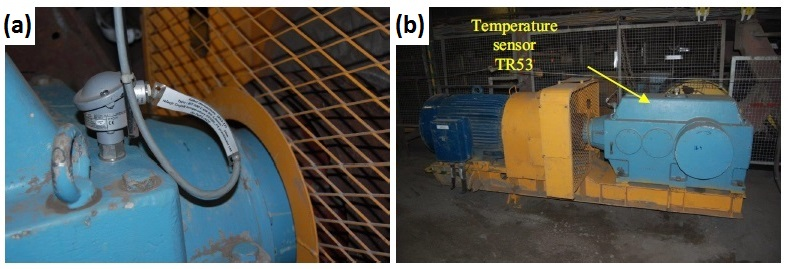
\includegraphics[width=0.9\textwidth]{machine_and_temperature_sensors.jpg}
\caption{A belt conveyor drive: a temperature sensor location (a), an electric motor, a coupling and a gearbox (b) }
\label{fig:machine}
\end{figure}


%\begin{figure}

%\centering
%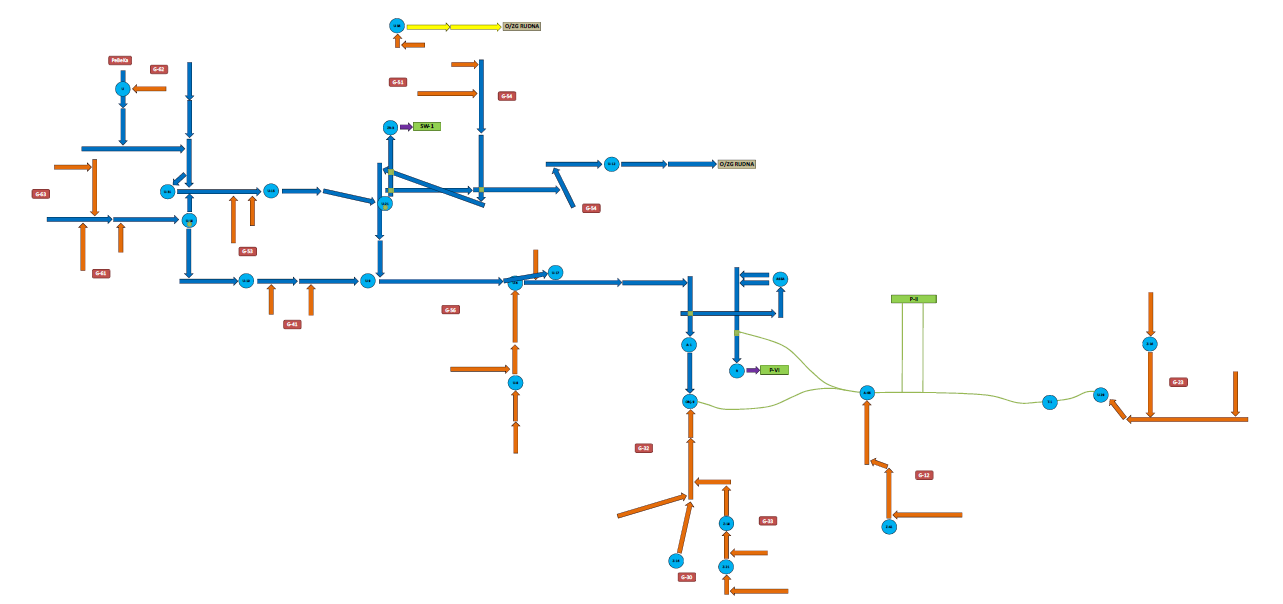
\includegraphics[width=0.9\textwidth]{ZGPS_conveyor_system.png}
%\caption{The conveyor system in KGHM OZG Polkowice-Sieroszowice mine. Each elementary segment is a separate conveyor, scale of the system makes frequent inspection difficult.}
%\label{fig:conveyor_system}
%\end{figure}
%\begin{figure}



\begin{figure}

\centering
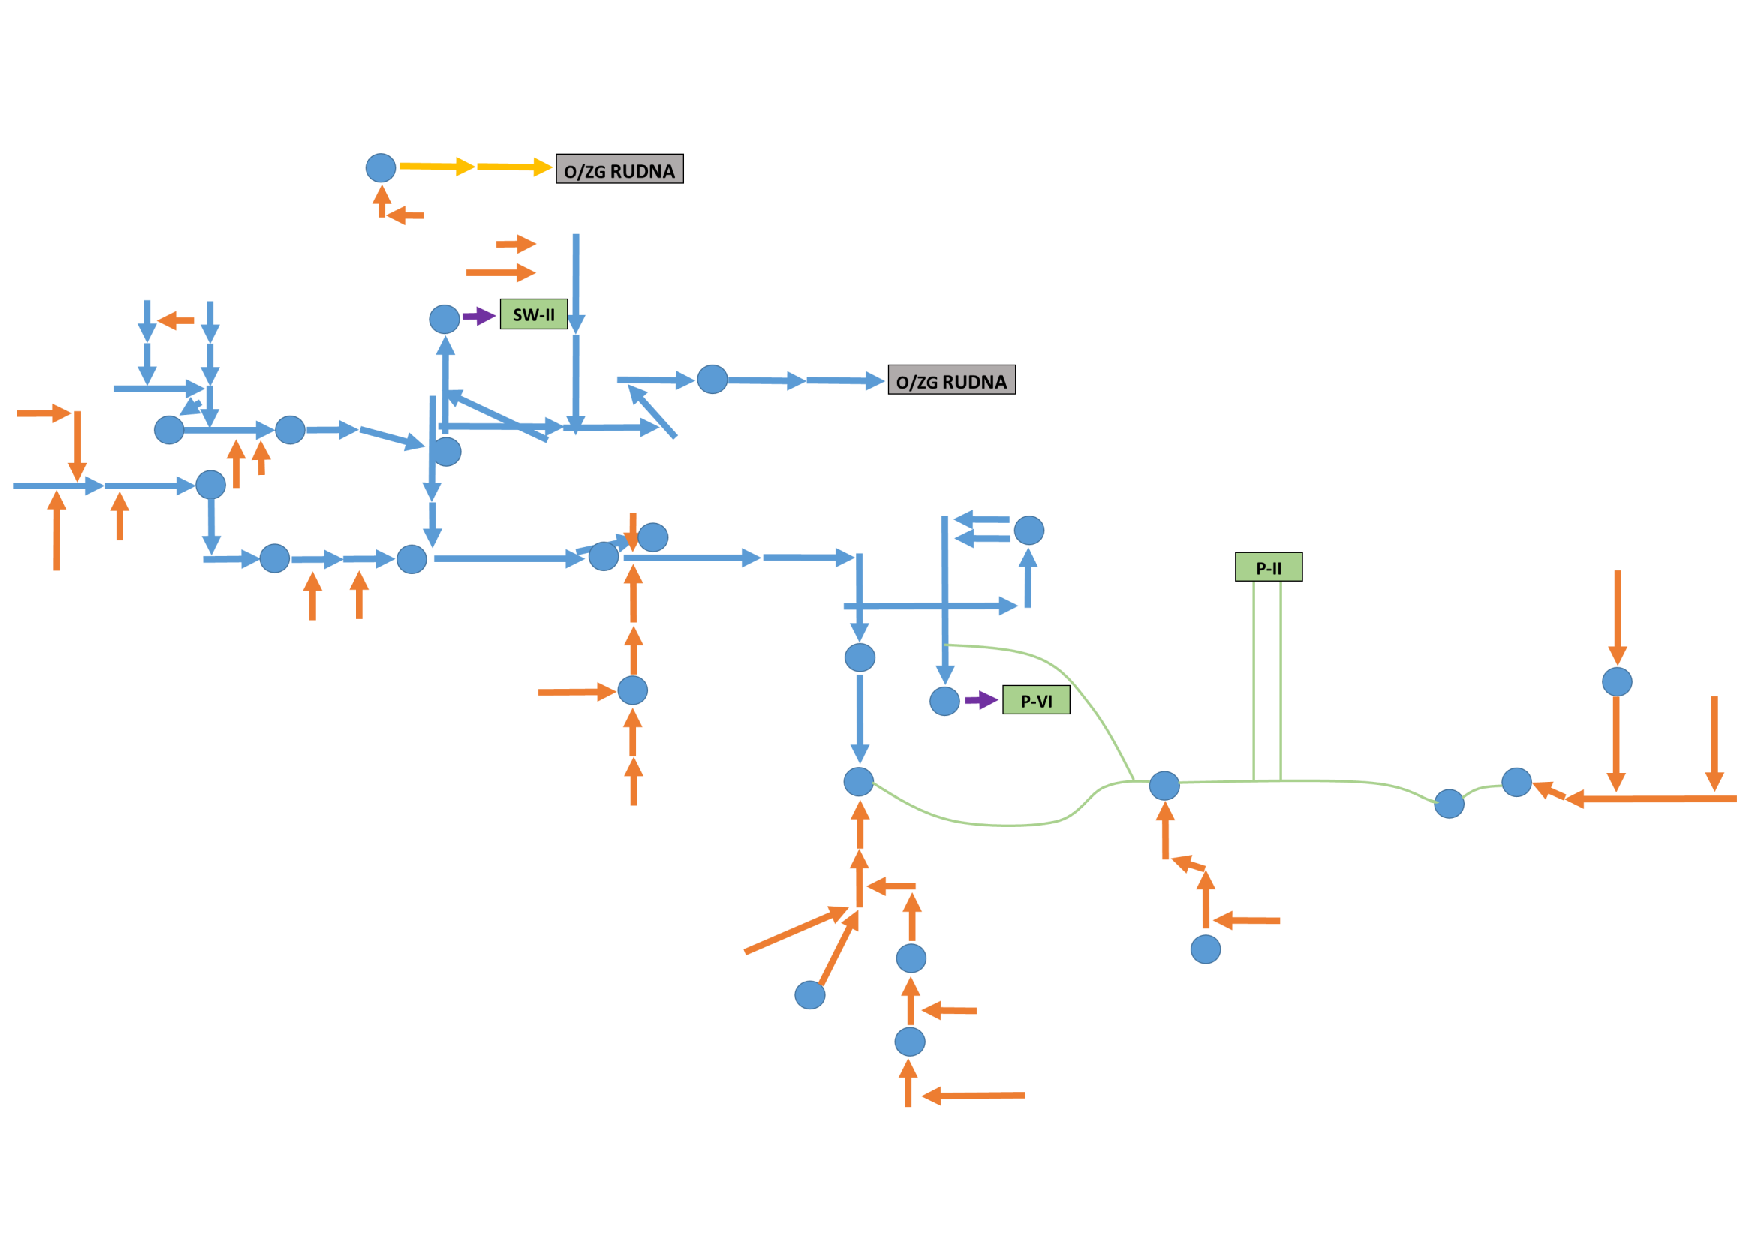
\includegraphics[width=0.9\textwidth]{ZGPS_conveyor_system.pdf}
\caption{The conveyor system in KGHM OZG Polkowice-Sieroszowice mine. Each elementary segment is a separate conveyor, scale of the system makes frequent inspection difficult. Each arrow means conveyor, each circle bunker for ore storage.}
\label{fig:conveyor_system}
\end{figure}




%\centering
%\includegraphics[width=0.9\textwidth]{rudna.png}
%\caption{The conveyor system in KGHM OZG Polkowice-Sieroszowice mine} \textcolor{red}{musimy miec lepszy rysunek}
%\label{fig:conveyor_system}
%\end{figure}
%\begin{figure}

%\centering
%\includegraphics[width=0.9\textwidth]{all.jpg}
%\caption{The conveyor system in KGHM OZG Polkowice-Sieroszowice mine} \textcolor{red}{musimy miec lepszy rysunek}
%\label{fig:conveyor_system}
%\end{figure}


\begin{figure}[ht!]
\centering
\begin{minipage}[c]{0.48\textwidth}
\centering
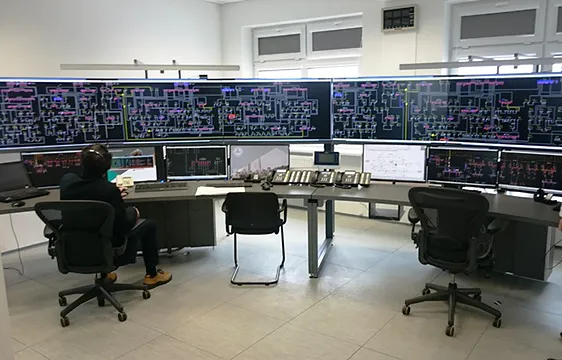
\includegraphics[width=0.8\textwidth]{One_control_Room_ZGPS.png}
\caption{One Control Room in KGHM OZG Polkowice-Sieroszowice mine (source: http://polskamiedz.wp.pl/artykul/kopalnie-kghm-jak-w-filmowym-avatarze-gornik-pod-ziemia-najmniej-potrzebuj-dzis-kilofu} 
\label{fig:One_control_Room_ZGPS}
\end{minipage}
\hfill
\begin{minipage}[c]{0.48\textwidth}
	\centering
	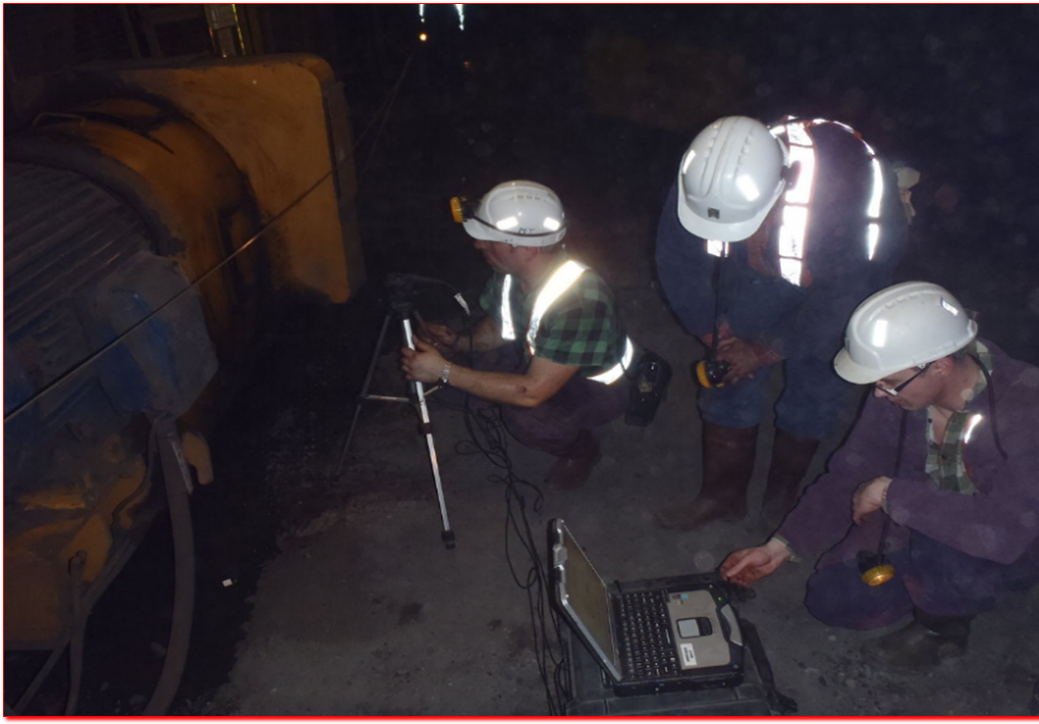
\includegraphics[width=0.8\textwidth]{inspection2.png}
	\caption{Intervention of the inspection team}
	\label{fig:inspection2}
	\vspace{1.5cm}
	\end{minipage}
\end{figure}

While monitoring of drive units is almost solved thanks to SCADA or occasional detailed inspections, unfortunately supervision of the elements of the conveyor route is still a challenge. It should be done regularly, as various components may be damaged or simply may require some corrections. Thanks to the Internet of Things (IoT) concept, some authors proposed solutions based on distributed smart sensors network, but taking into account the number of idlers to be monitored, slow development of wireless transmission system in underground mine, reliability of such solutions, etc., there is a need to search for more realistic/practical scenarios \cite{LIU2018277}. 

One of the most critical issues is friction between stationary elements and moving belt, as well as increased rolling resistance of idlers supporting the belts. Research on idlers is an important topic in belt conveyor exploitation and maintenance \cite{krol_diagnostyka, krol_miningscience}. Damaged idlers may be a source of increased energy consumption or even initiate belt damage or fire. So, to avoid catastrophic failures, a visual inspection is performed by miners along the conveyor route \ref{fig:BCS_ispection}. Note, (see Fig \ref{fig:conveyor_system} that there are tens of kilometers of conveyors and they should be checked from both sides. It requires human resources, takes time and it is pretty risky for people. The idea of using mobile robots for inspection is not a new one. There are some promising papers on that subject \cite{8461191,8621649,6462974,932642,1507481}. Several inspection scenarios have been defined under the umbrella of THING project \cite{zimrozMPES2019}. Interesting examples of using inspection robots in underground mine is mapping or exploration \cite{li_savkin_vucetic_2020,8990018,8741532,1371614,Grehl2015,6743612}, supporting of rescue action \cite{5069840,5563599,6685501,5069840} or other "mine disasters" \cite{5420386}.

\begin{figure}[ht!]
	\centering
	\includegraphics[width=\textwidth]{INSPECTION.png}
	\caption{Conveyor belt route inspection nowadays}
	\label{fig:BCS_ispection}
\end{figure}

In this paper we will propose a UGV (Unmanned Ground Vehicle) platform as a virtual miner that will do the same work as inspection staff, namely it will ride along the belt conveyor and collect information about conveyor operation using sensors. In section 2, we will provide a brief description of the robotic platform. Section 3 contains the use case description - an experiment in our laboratory where the belt conveyor test rig is located. We also provide a plan and results of our experiments. Section 4 contains the methods and results of inspection data analysis. Finally, sections Discussions and Conclusions are provided.


\section{A UGV platform}\label{meth} 

A developed mobile robot belongs to the UGV (Unmanned Ground Vehicle) class of systems. The frame has been assembled using light aluminum construction rails. Drive block has been installed in the front part, and the back contains the cargo space connected with the front using the two-axial joint (fig. \ref{robot_scheme}). It allows for all of the wheels to make contact with the ground all the time, amidst the stiff suspension. Additionally, such a solution has good stability (Fig. \ref{fig:robot_fig}).



\begin{figure}[ht!]
\centering
\begin{minipage}[c]{0.48\textwidth}
\centering
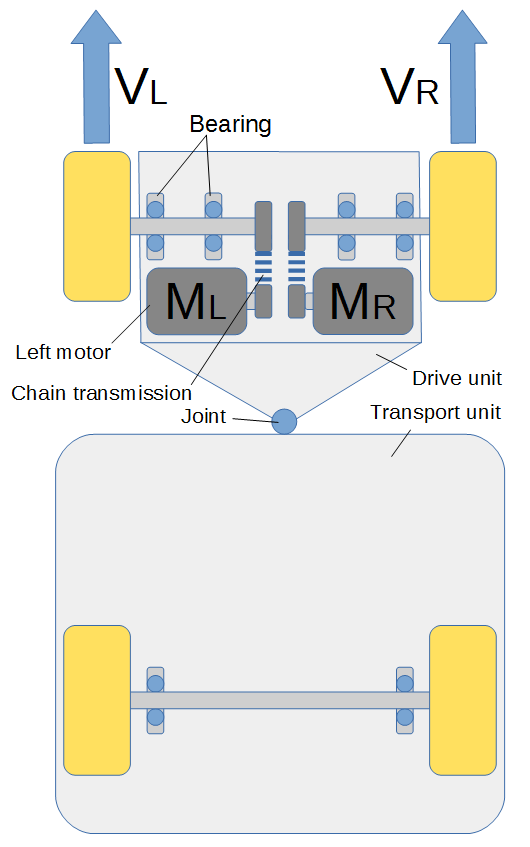
\includegraphics[width=0.6\textwidth]{Robot_scheme.png}
\caption{A scheme of the chassis of the robot for inspection in underground mine}
\label{robot_scheme}
\end{minipage}
\hfill
\begin{minipage}[c]{0.48\textwidth}
\centering
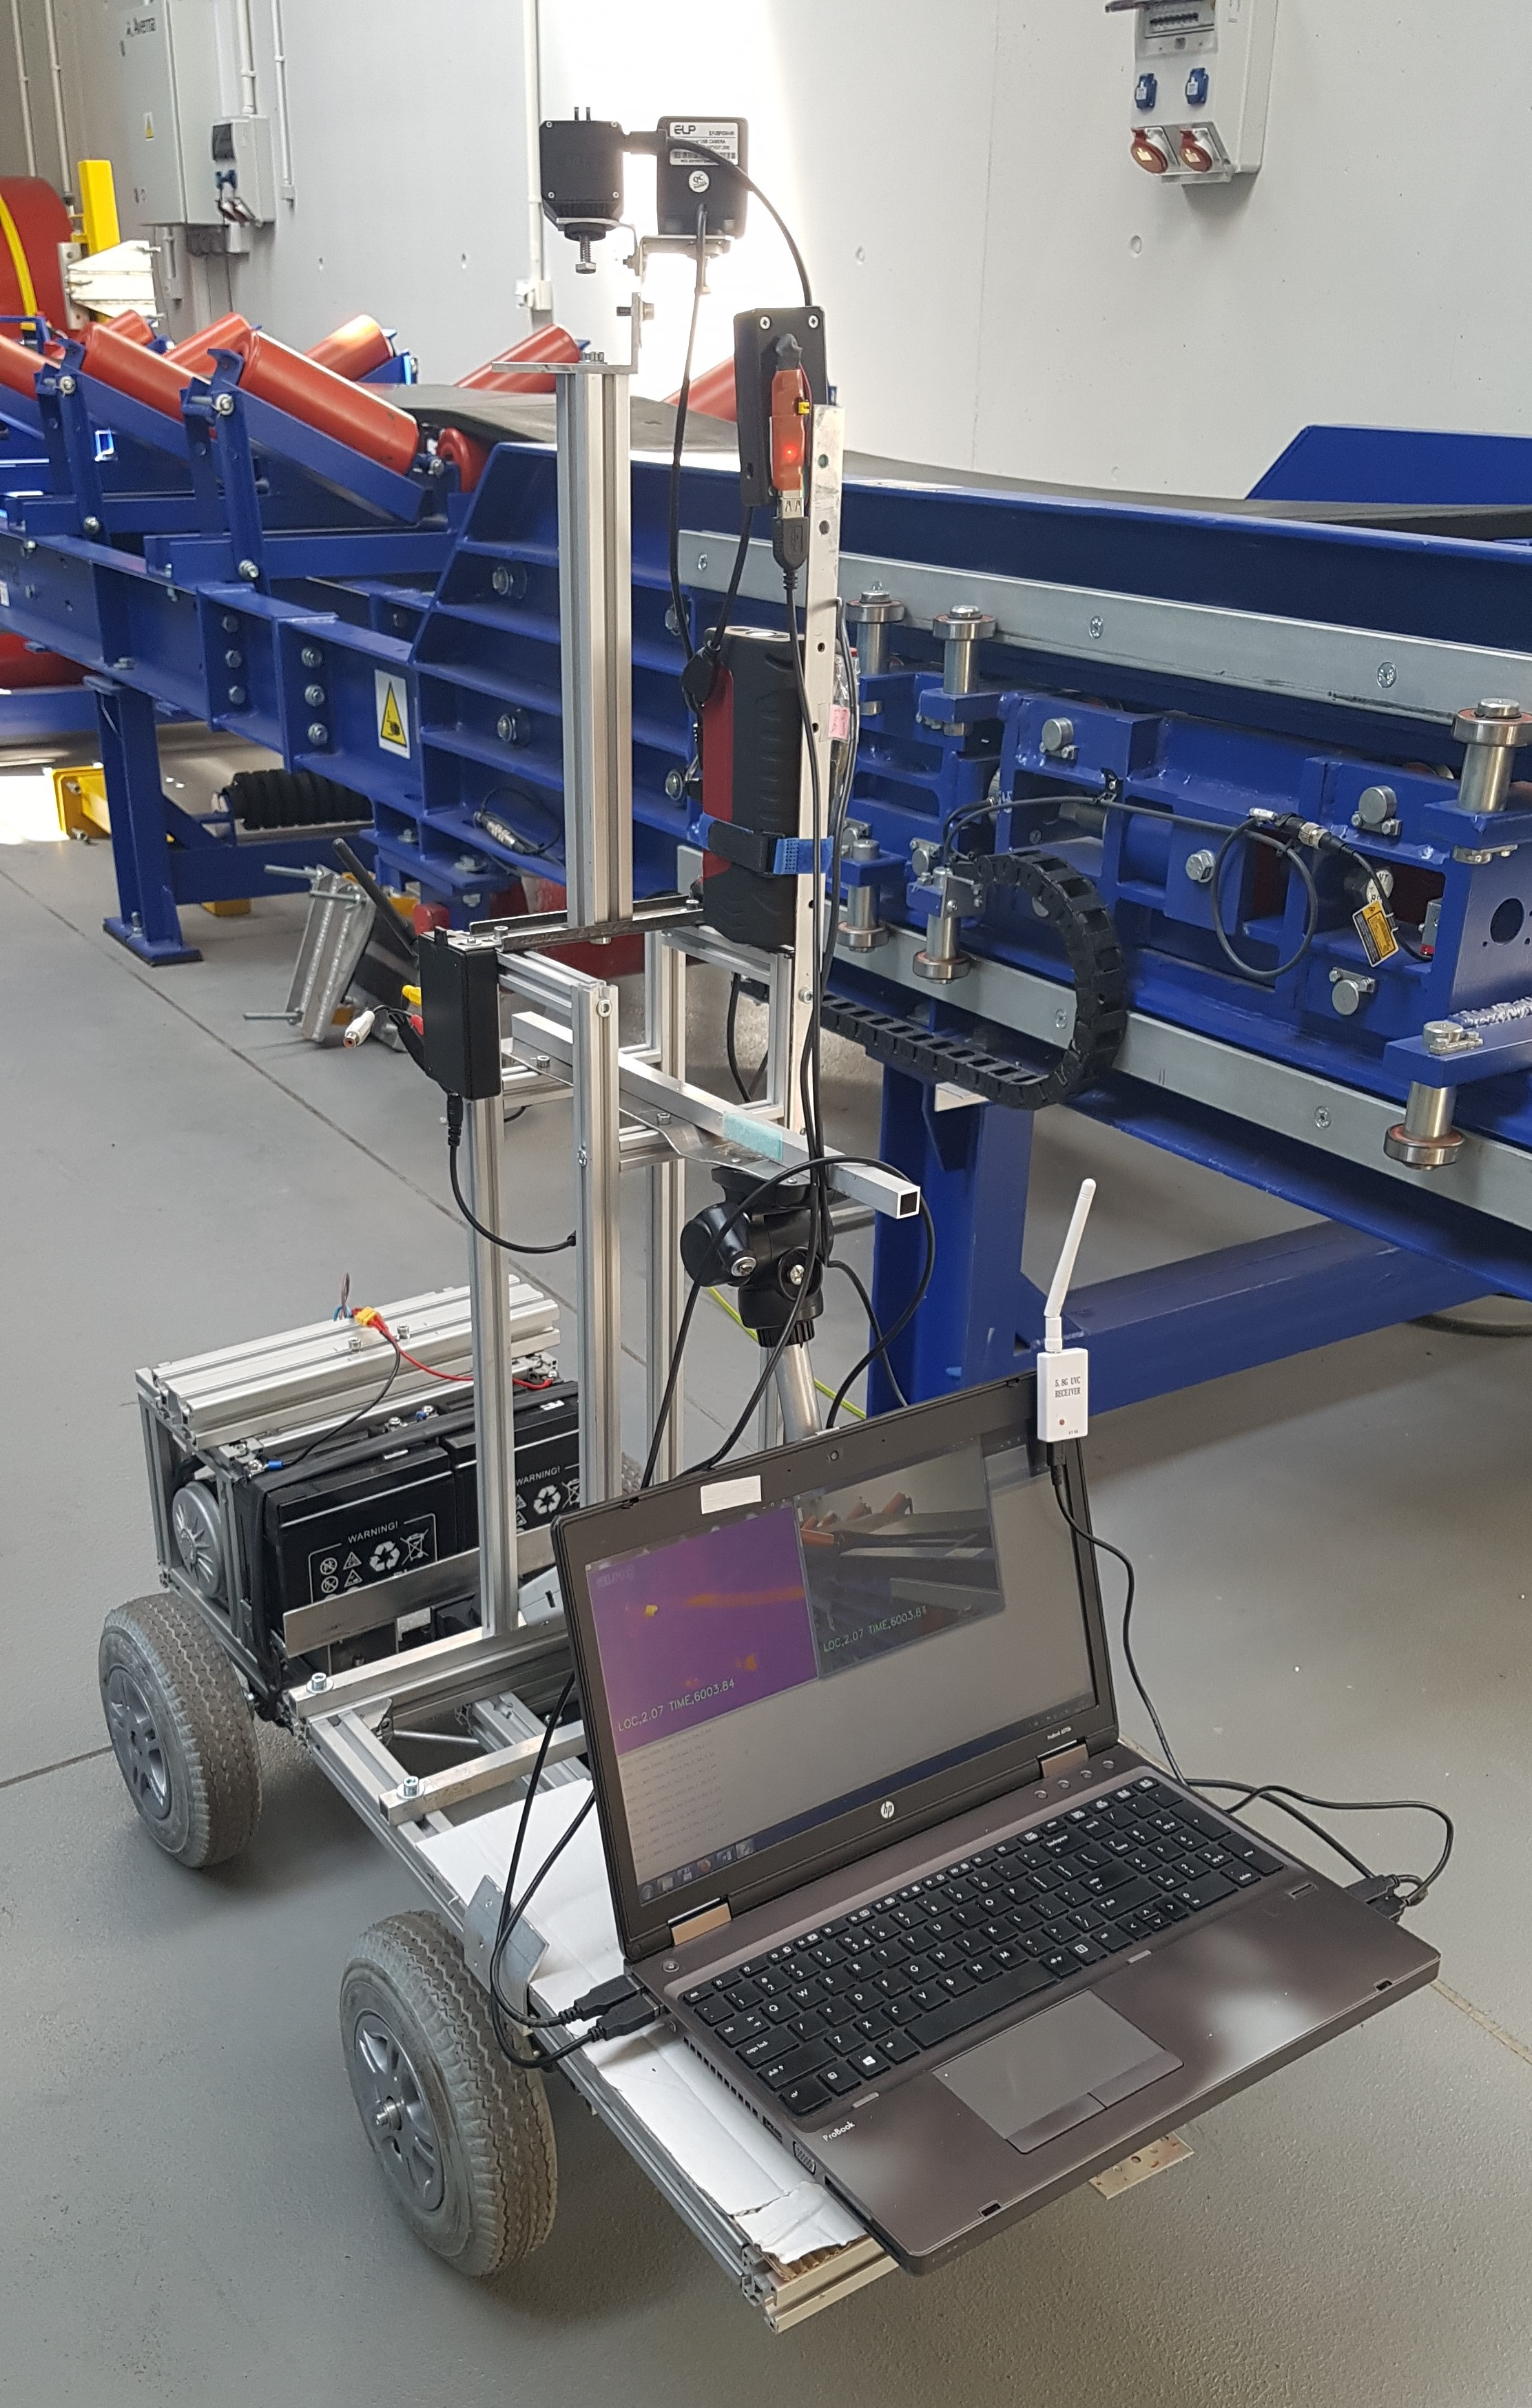
\includegraphics[width=0.6\textwidth,  height=\textwidth]{robot.jpg}
\caption{A robot for belt conveyor inspection.}
\label{fig:robot_fig}
\end{minipage}
\end{figure}

The wheels are driven by 24V 250W DC motors integrated with a cylindrical gearbox with 19:1 ratio. Additional reduction and power transmission are achieved by using chain and cogwheels as an intermediate step. The driving system is a classic 2.0-class structure. Maneuvering is performed by applying the difference in speeds of the wheels. The robot is powered by two 12V batteries with 12Ah capacity each. Voltage for powering the electronics (5V) is obtained by using a step-down transformer.


\subsection{Control system of the mobile platform}
The robot control is presented in fig. \ref{fig:Robot_Control}. Driving the robot is performed by controlling the speed of the wheels using PWM (Pulse Width Modulation) signals as well as direction signal from the ATMega 328p micro-controller in the standard Arduino Nano module. PWM signal travels to the motors via H-bridges powered by additional relay enabling power cutoff (remotely or in case of an emergency stop). Motor current measurement system has been implemented in the driver to monitor the potential overload \cite{RobotRex}. The implementation of the control system is visible in Fig.  \ref{fig:front}. 
\begin{figure}[ht!]
%author={Jaroslaw Szrek and Pawel Wojtowicz}, 


\centering
\begin{minipage}[c]{0.48\textwidth}
\centering
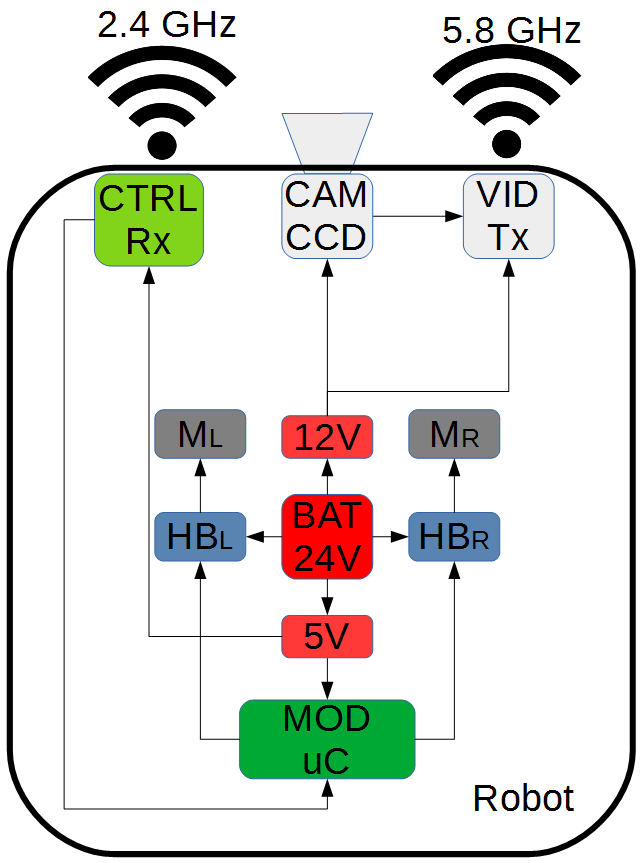
\includegraphics[width=0.9 \textwidth]{Robot_Control.png}
\caption{A concept of control system}
\label{fig:Robot_Control}
\end{minipage}
\hfill
\begin{minipage}[c]{0.48\textwidth}
\centering
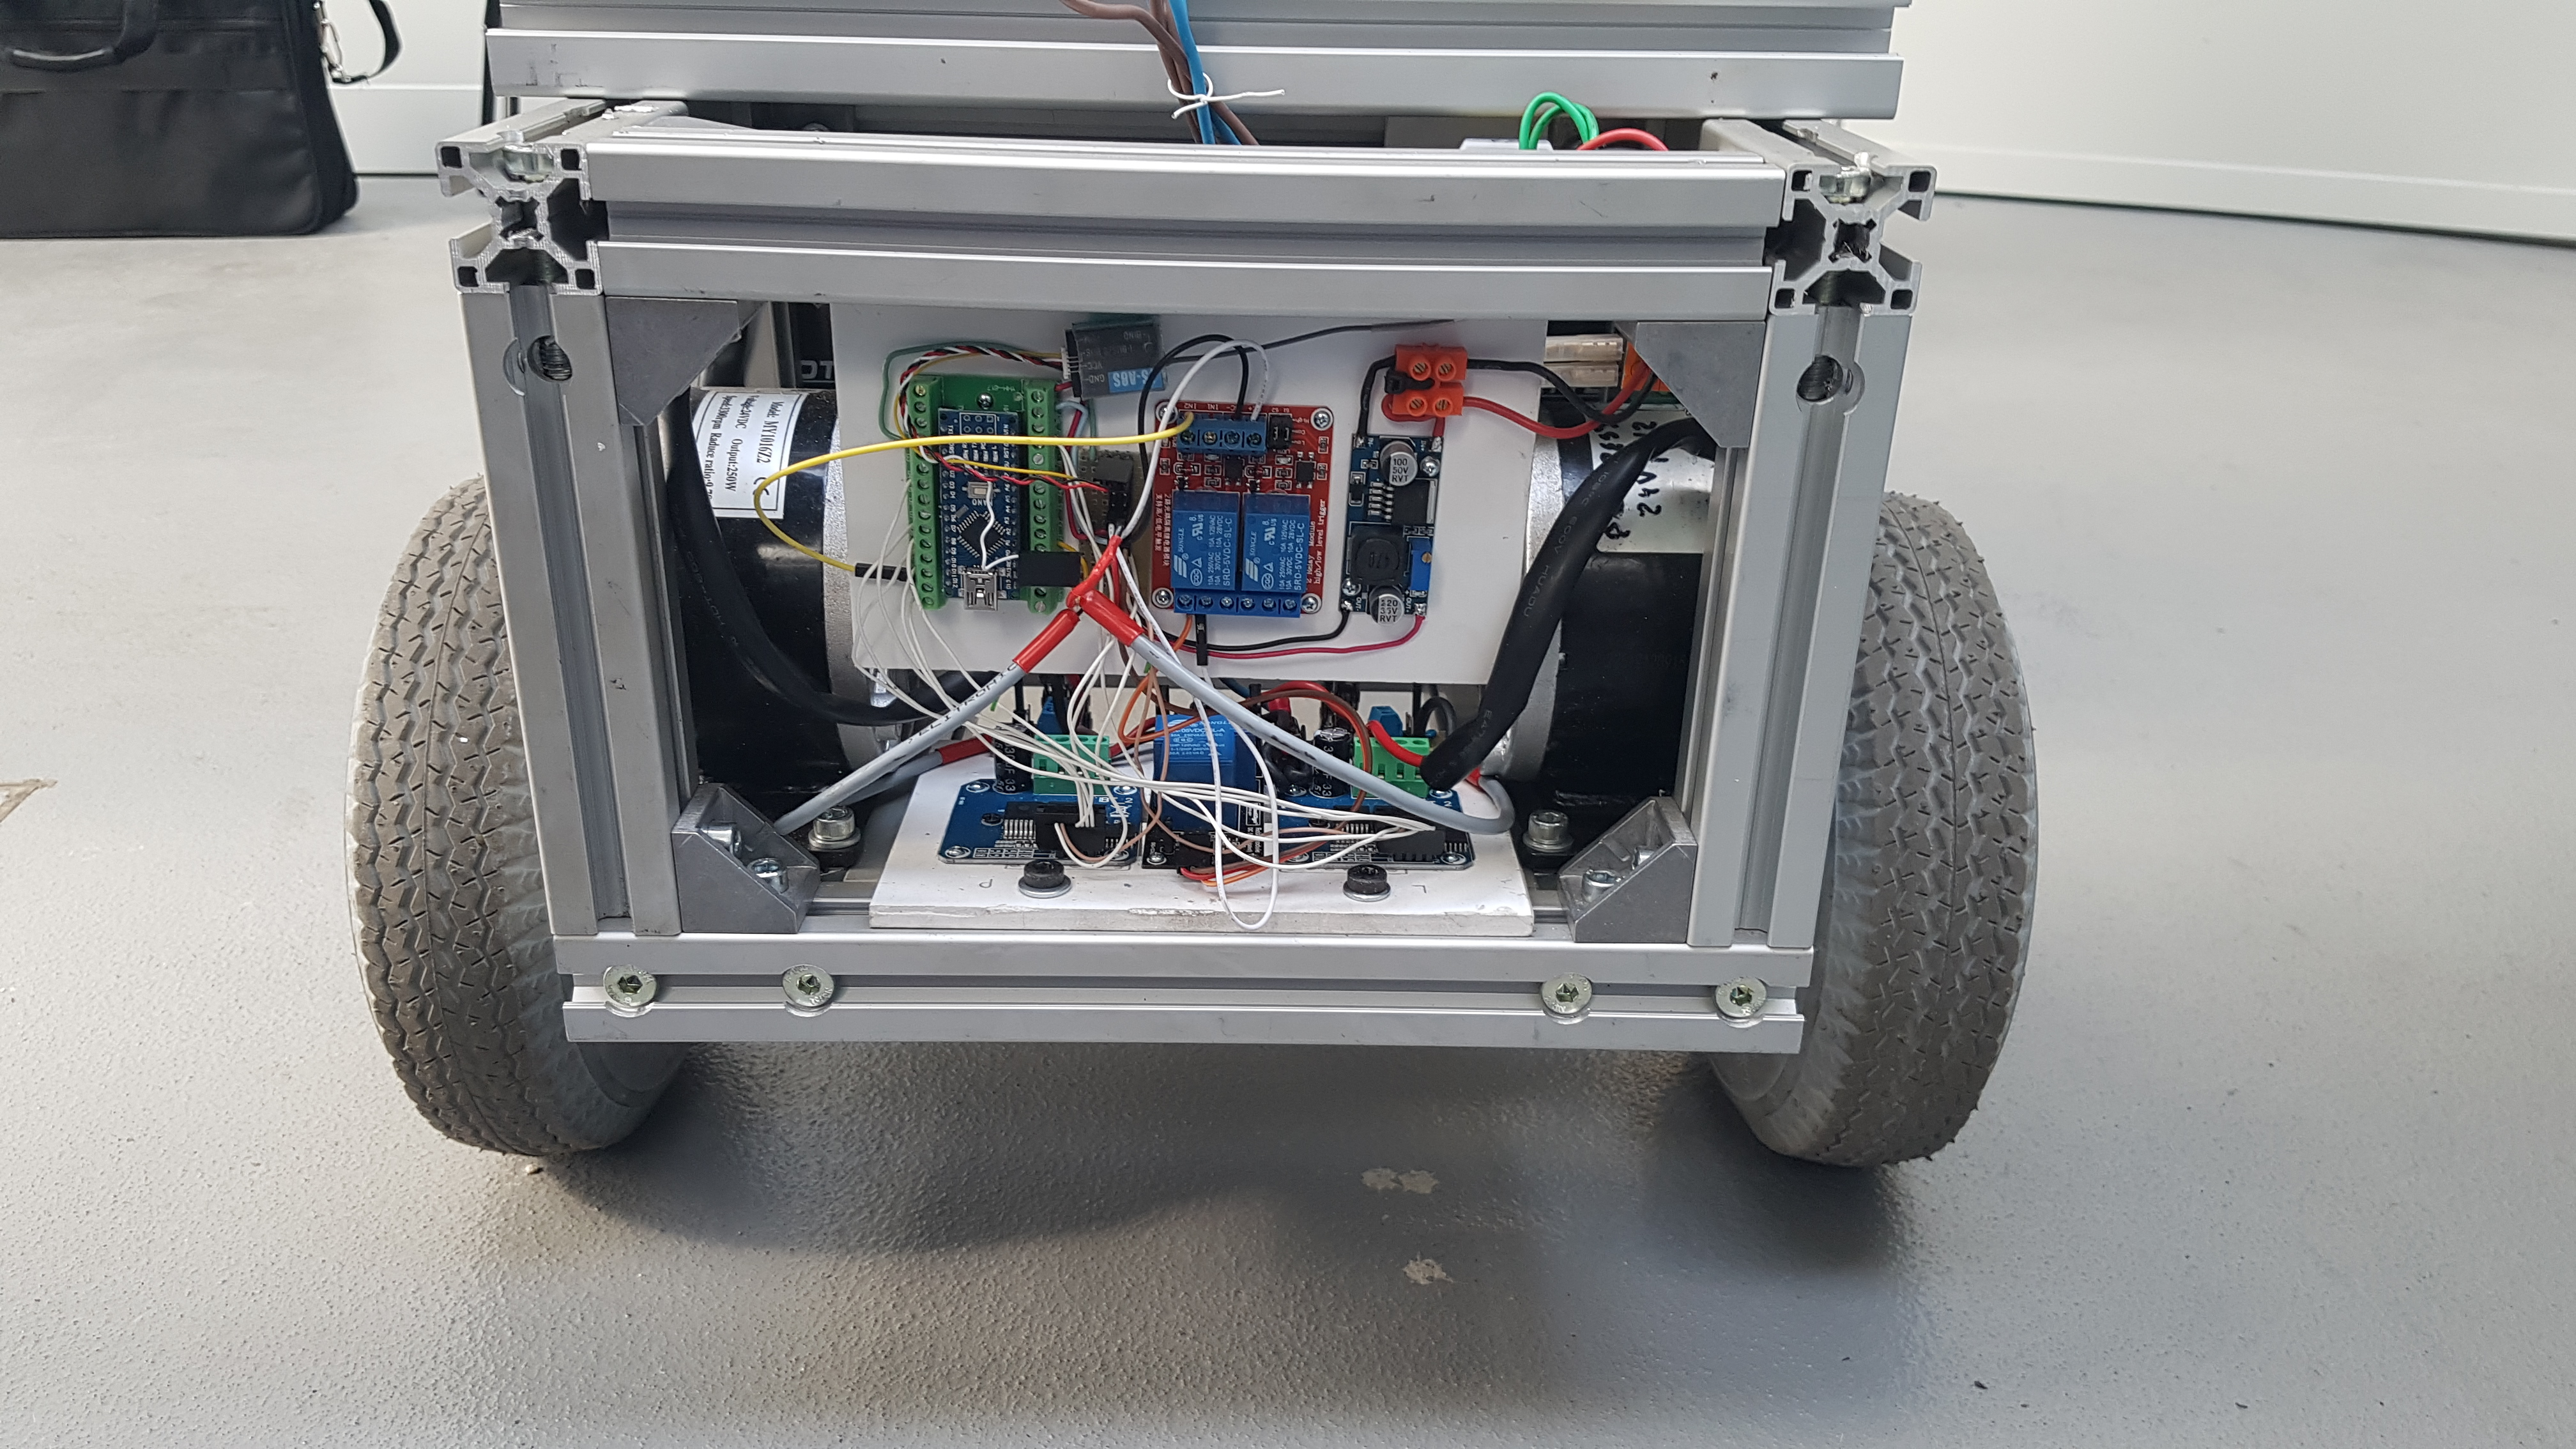
\includegraphics[width=0.9\textwidth]{front.jpg}
\caption{Hardware of control system}
\label{fig:front}
\end{minipage}
\end{figure}

An additional camera has been used to watch the area in front of the robot for manual steering. The video feed is wirelessly transmitted using a selected channel at the frequency of 5.8 GHz to remote control panel \cite{RobotLeg}. 

The operator steers the robot based on the video feed from the camera displayed on the external monitor, sending PPM (Pulse Position Modulation) wireless control signals from the remote manipulator via an independent 2.4 GHz band. The remote control panel structure is presented in Fig. \ref{fig:Robot_Control_panel}. 

\begin{figure}[ht!]
	\centering
	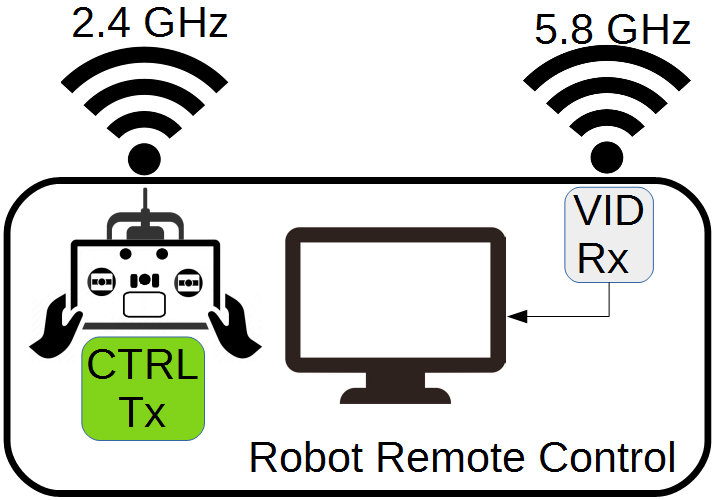
\includegraphics[width=0.4\textwidth]{Remote_Control.png}
	\caption{Mobile platform remote control panel}
	\label{fig:Robot_Control_panel}
\end{figure}

\subsection{Robot localization system.}
During the inspection it is important to precisely localize the place where a fault occurred. One of the systems that are precise enough for event localization is GPS. It can be successfully used for positioning in open space with high reliability and easy to use interface. However, in the case of underground mine there is no possibility for GPS communication in the underground conditions, so for such use case the Ultra-Wideband (UWB) transceivers have been proposed for the localization system (see Fig. \ref{fig:sensors}). 

\begin{figure}[ht!]
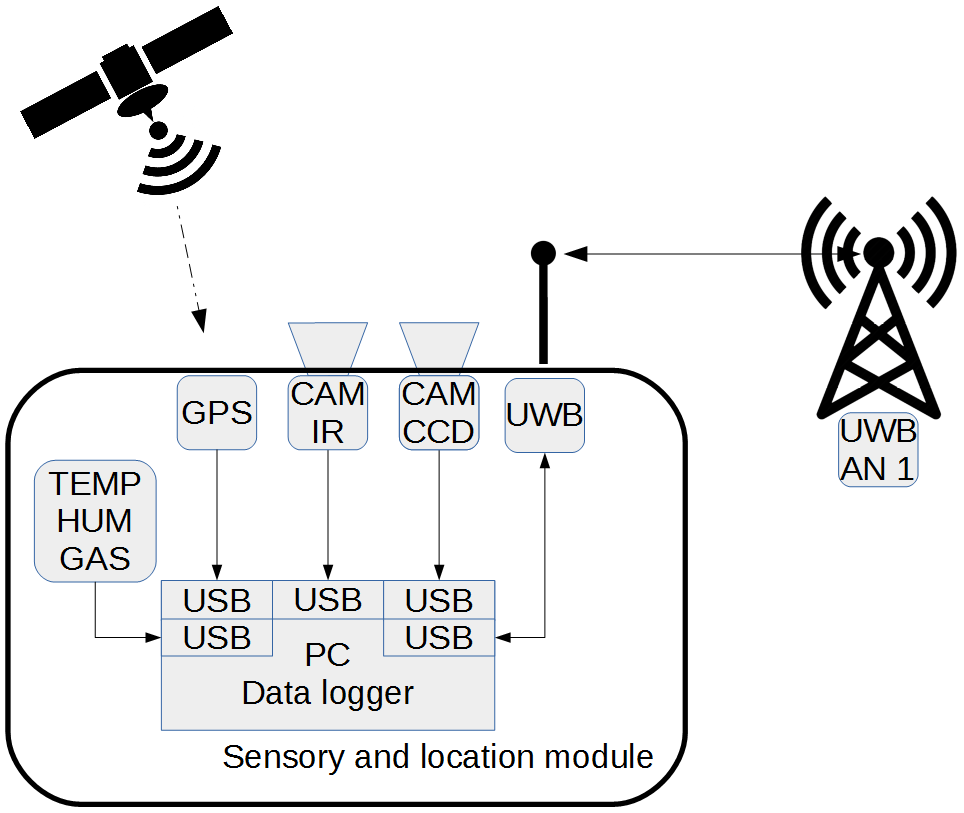
\includegraphics[width=0.7\textwidth]{Sensory_system.png}
\centering
\caption{Sensory and location module} \label{fig:sensors}
\end{figure}

The localization system is based on DWM1001 modules equipped with firmware, that ensures bi-directional distance estimation (TWR) and real-time localization system (RTLS). Inside the module, besides the system directly responsible for distance estimation (UWB Transceiver) there is also Bluetooth® Microprocessor Nordic nRF52832 and high-performance three-axis linear accelerometer with digital I2C/SPI serial interface standard output LIS2DH12 \cite{dwm1001}. Configuration of the module is realized via API interface which can be accessed using various interfaces such as UART, SPI, i2C, BT. Specific modules configured as Anchor (A) play a role of fixed beacons, and a module installed on the robot operates as a tag (T).


\begin{figure}[ht!]
	\centering
	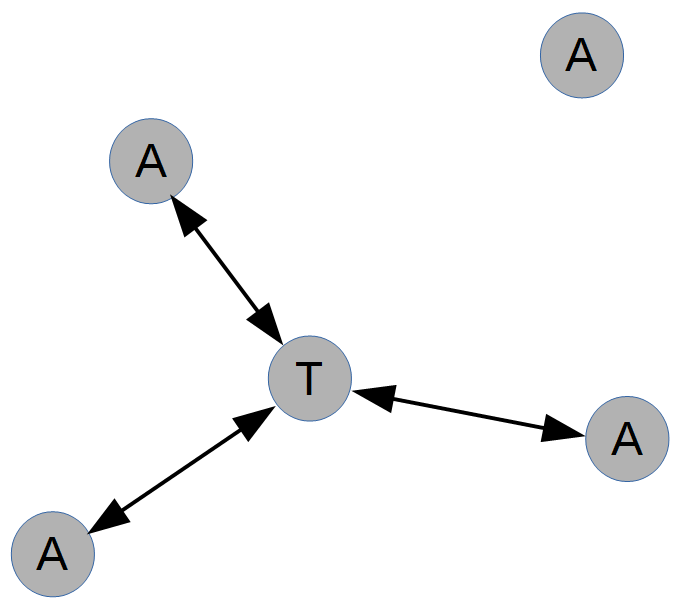
\includegraphics[width=0.4\textwidth]{RTLS_Tagi_Kotwice.PNG}
	\caption{Localization of Tag}
	\label{fig:RTLS}
\end{figure}

The bi-directional communication and data exchange between the modules as well as the known position in space of each anchor allows us to precisely calculate distances between them and using trilateration algorithms to estimate the position of a tag in space (see Fig. \ref{fig:RTLS}). 

The inspection itself is carried out by driving the robot along the conveyor keeping close distance to it. Deviation of the measurement system in a vertical direction with respect to the conveyor is expected to be minimal, probably negligible. Hence, the number of localization modules can be very limited.


\begin{figure}[ht!]
	\centering
	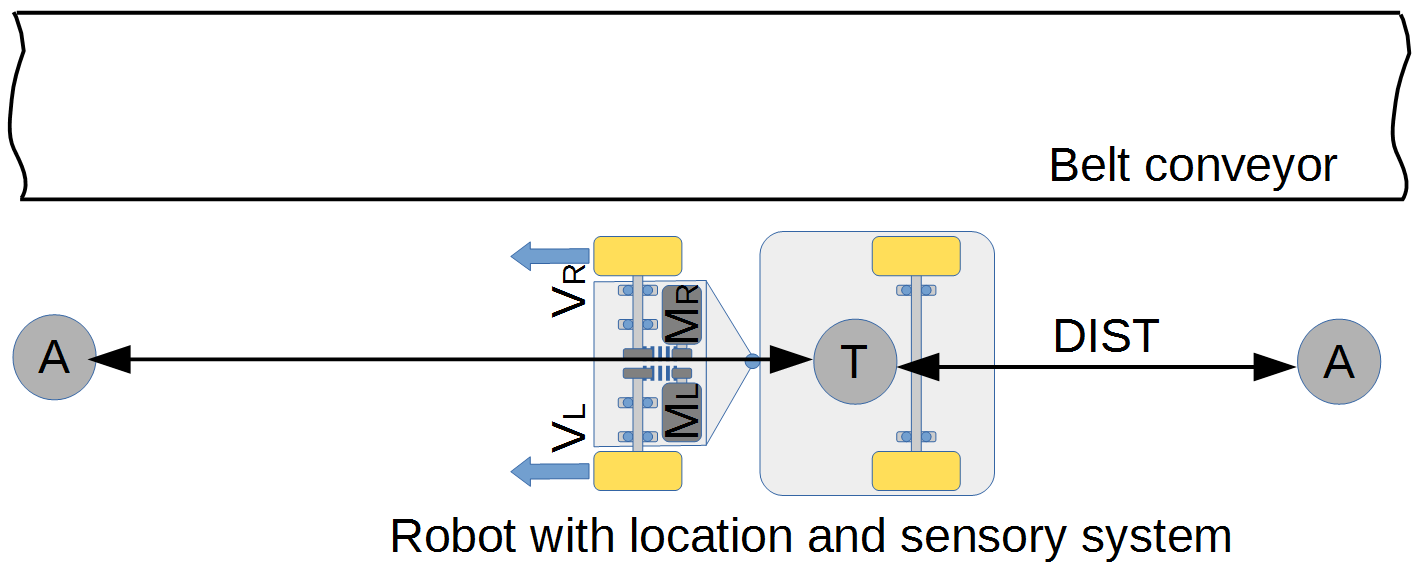
\includegraphics[width=0.7\textwidth]{RTLS_przenosnik_robot.PNG}
	\caption{A plan of the experiment in the lab}
	\label{fig:plan_exp}
\end{figure}

Modules configured as anchors have been installed along the conveyor in such spacing that a tag is always in the range of at least one of them, see Fig \ref{fig:plan_exp}. For the purpose of the experiment the beacon has been placed on a stand (Fig. \ref{fig:UWB_antena}). 

\begin{figure}[ht!]
	\centering
	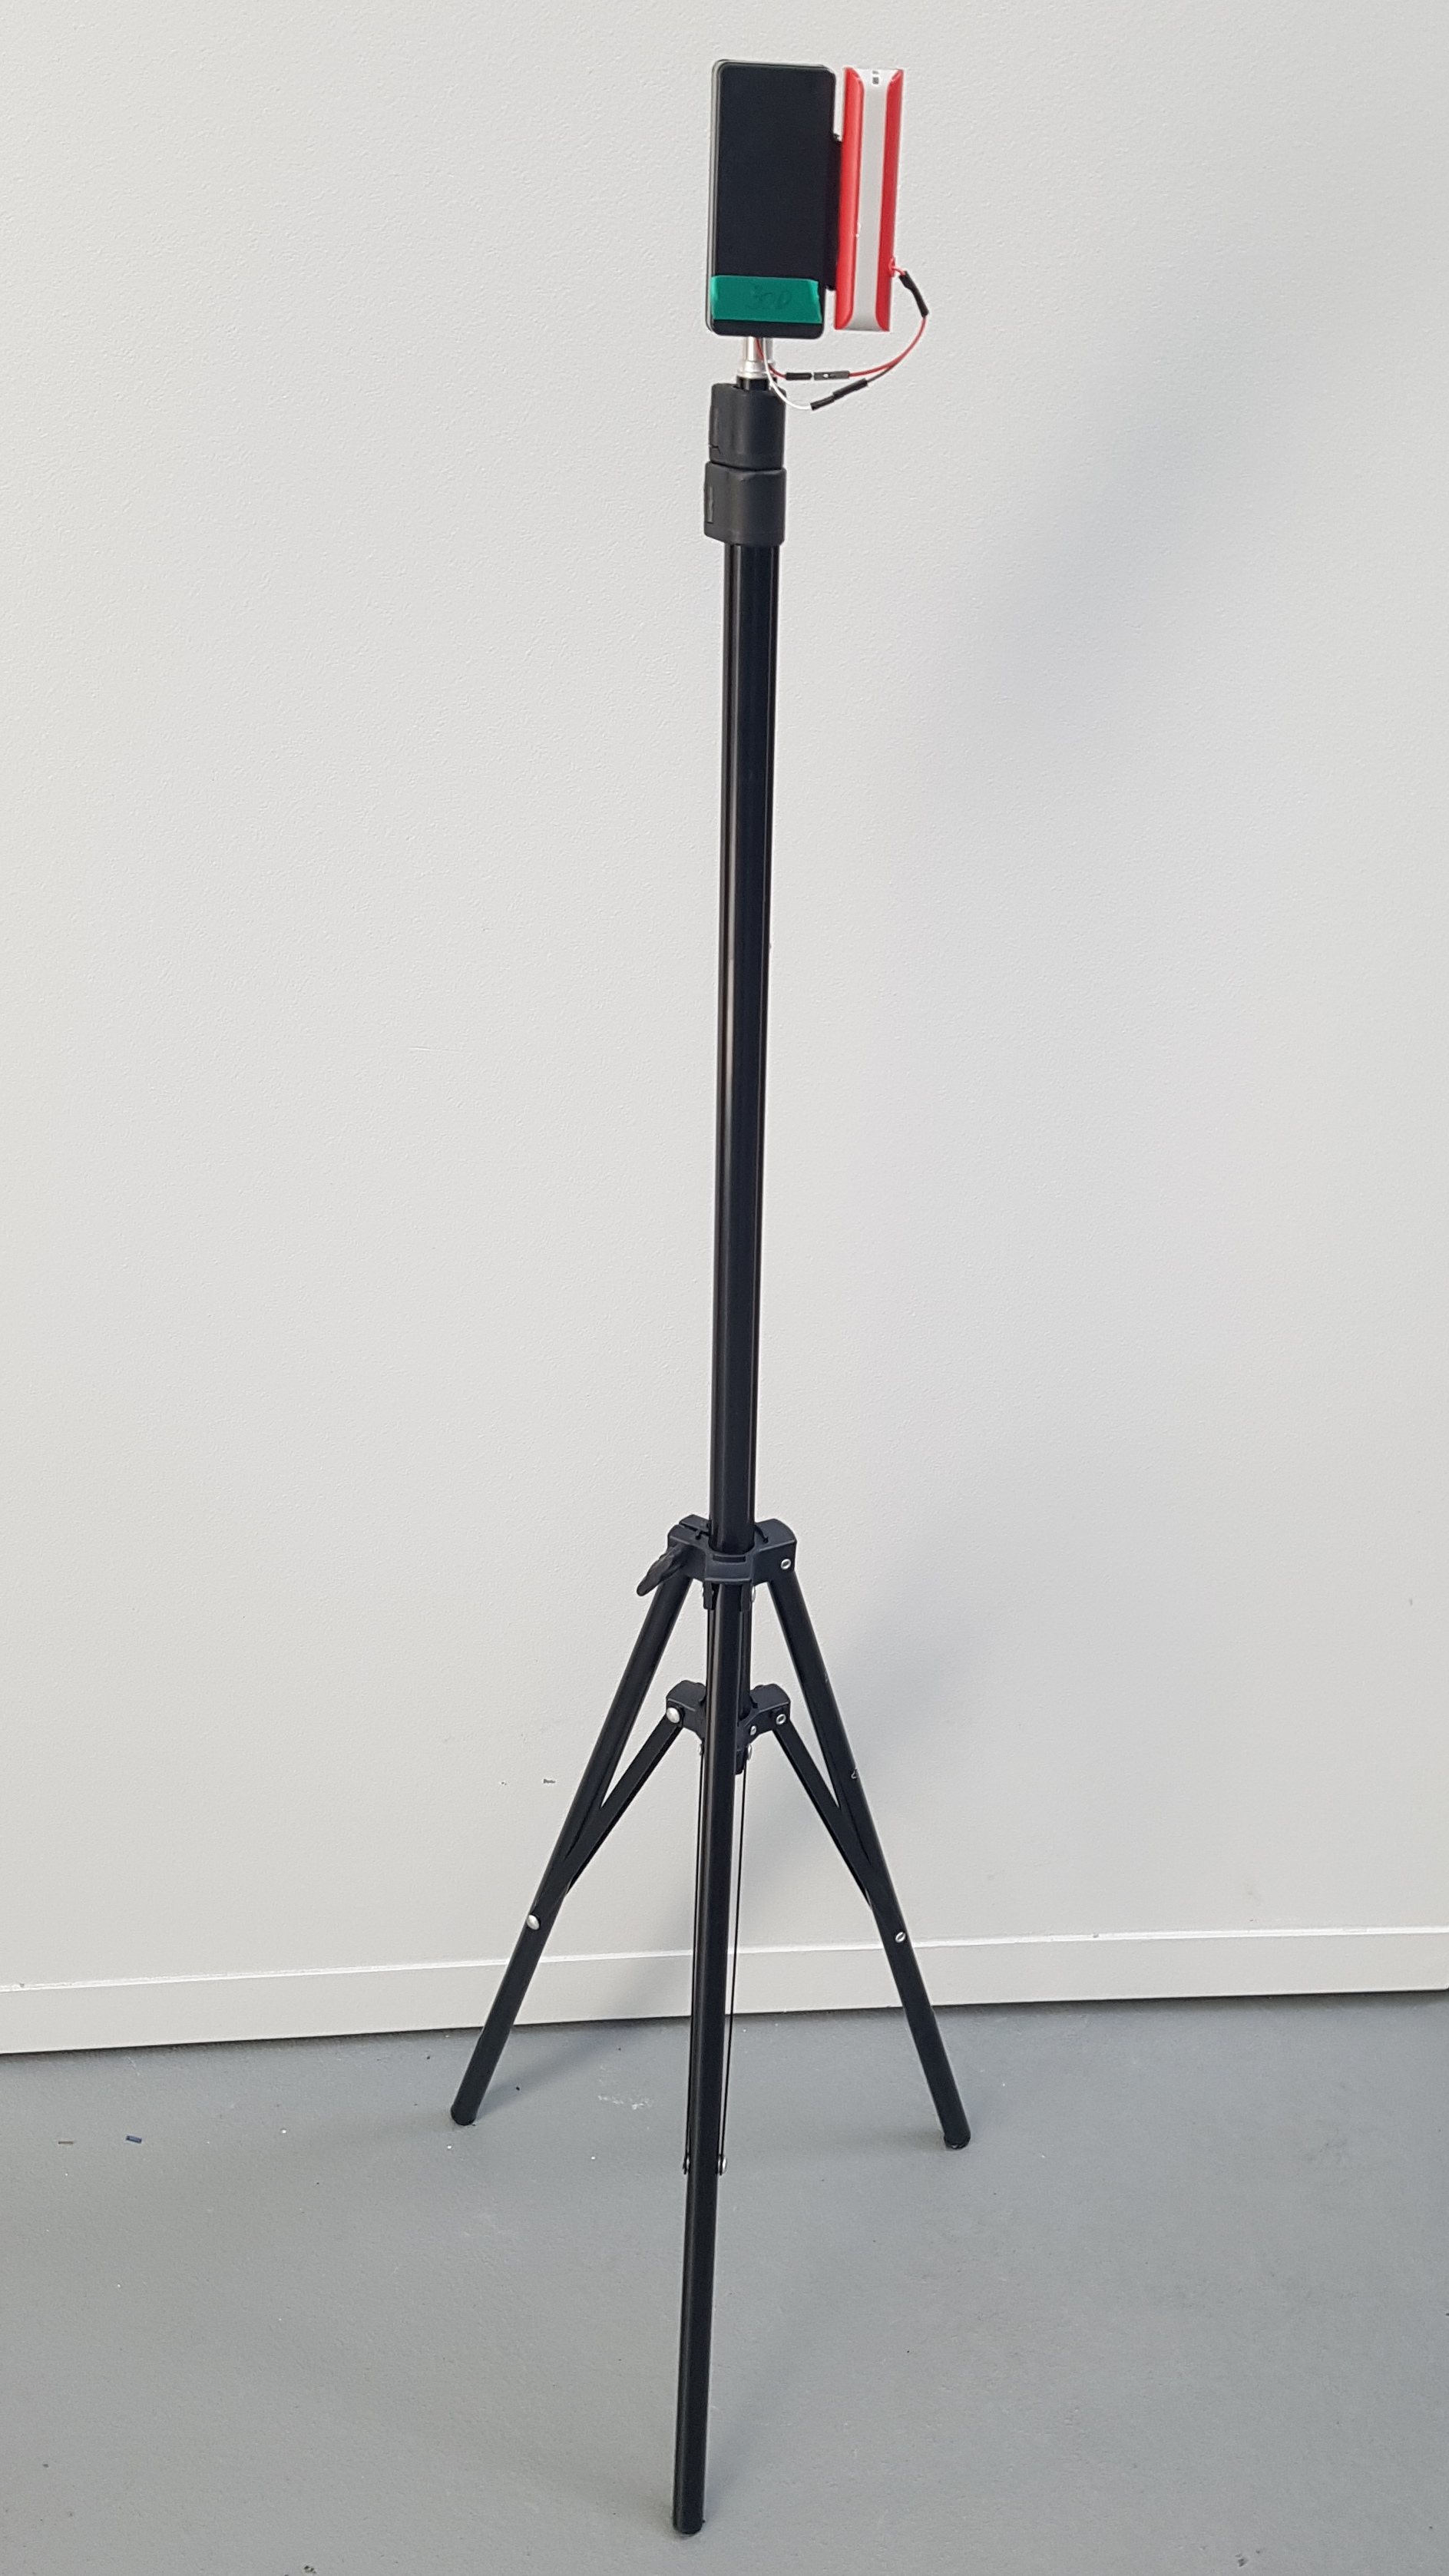
\includegraphics[width=0.4\textwidth]{gps.jpg}
	\caption{UWB anchor}
	\label{fig:UWB_antena}
\end{figure}
During the inspection the position relative to the unique antenna in parallel to the sensor data. Hence, it is possible to localize the place of any event. Using the proposed system it is possible to achieve an accuracy of 10 cm.


\subsection{Onboard sensors}

While at the moment the authors focus on hotspot detection based on thermal imaging, it is planned to equip the robot with an extensive sensor suite. Considering the fact that the final result of the diagnostic mission is the ability to provide all the necessary information to the maintenance crew and actually send people to the location, it is important to ensure that the environment is safe for them to arrive. Hence, it is crucial to be able to monitor additional parameters, such as air temperature and humidity, the concentration of dangerous gases such as CO, H$_2$S or NO$_x$, or the velocity of air current (some corridors are used for ventilation and air currents can be really strong). Besides the safety parameters, an inspection of other features is planned (i.e. idler set dislocation or internal faults such as defects of bearings possible to be detected via vibroacoustic data analysis). 

To address those needs, besides the already present thermal and visual cameras, it is planned to equip the robot with sensors such as LIDAR, gas concentration sensors, temperature and humidity sensors, air velocity sensor and a microphone for noise measurements.

The algorithm for reading and recording sensory data is shown in Fig. \ref{fig:Algorytm_cam_loc}. The application works in two threads. One thread corresponds to the reading of location data, the other thread for reading data from cameras.

% \begin{figure}[ht!]
% 	\centering
% 	\includegraphics[width=0.7\textwidth]{INSPECTION.png}
% 	\caption{conveyor belt route inspection nowadays}
% 	\label{fig:BCS_ispection}
% \end{figure}






% to my mozemy powiedziec z Jackiem czego potrzebujemy
% to otwarta platforma
% lidar, vizja, termo, gaz, temperatura, wilgotnosc, predkosc przeplyywu powietrza, halas 

\begin{figure}[ht!]
	\centering
	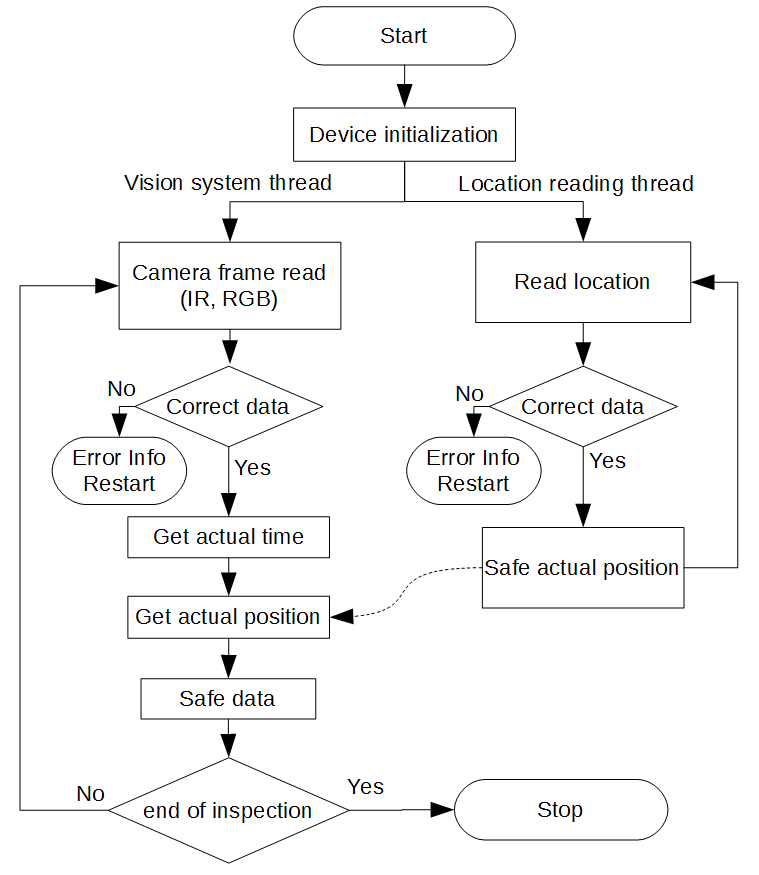
\includegraphics[width=0.6\textwidth]{Alg_cam_loc_reader.png}
	\caption{Reading and recording of sensory data algorithm}
	\label{fig:Algorytm_cam_loc}
\end{figure}




\subsection{Inspection data analysis module}

At the current stage of development the inspection is focused on hotspot detection using thermal imaging. Data analysis is carried out offline (ultimately to be carried out in real-time during the inspection). First, the image is acquired, then the threshold based on color is performed. When the detected area has a sufficiently large surface, a message is generated. Besides, the event view along with the location is saved and forwarded for verification by the service team. The algorithm was implemented in Python using the OpenCV library \cite{opencv}, and the general flowchart is presented in Fig. \ref{fig:alg_hot_detection}.

\begin{figure}[ht!]
	\centering
	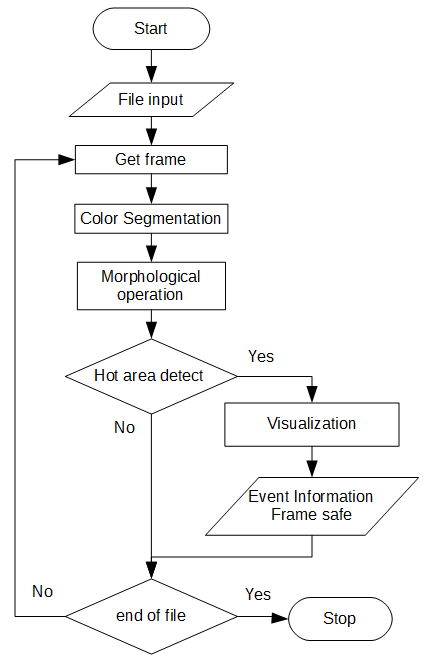
\includegraphics[width=0.5\textwidth]{Alg_cam_hot_point_detection.png}
	\caption{An algorithm of hot area detection}
	\label{fig:alg_hot_detection}
\end{figure}



\subsection{Data transmission and recording}

Data acquisition and transmission take place in parallel using several channels. Thermal and RGB images are registered locally within the board computer. Additionally, together with the vision, the robot position relative to the localization system and time information is recorded, which allows us to synchronize two independent camera feeds, as well as identify the event location such as a fault. To confirm the correctness of the view, it is possible to see the camera feed via WiFi (for example using remote desktop). Downloading of the data takes place after the mission ends. 

The structure of the system is prepared in a way that it is possible to conduct a mission autonomically, however, in the early stage of the development the robot works in teleoperation mode. Further publications will describe more results related to autonomous applications.

\newpage
\section{The use case description}\label{meth} 


\subsection{A belt conveyor test rig}

The biggest belt conveyor research center in Europe is located in the GEO3EM Research Center at the Wroclaw University of Technology, Faculty of GeoEngineering Mining and Geology. One of the available test rigs is a 7m belt conveyor test rig with artificially introduced belt damages, idlers in different conditions and ability to work under various belt speeds (\ref{beltconveyor}). This test rig has been developed for research related to belt conveyor diagnostics and maintenance. In this paper, we have used this test rig to investigate the application of mobile inspection robot (UGV).


\begin{figure}[ht!]
	\centering
	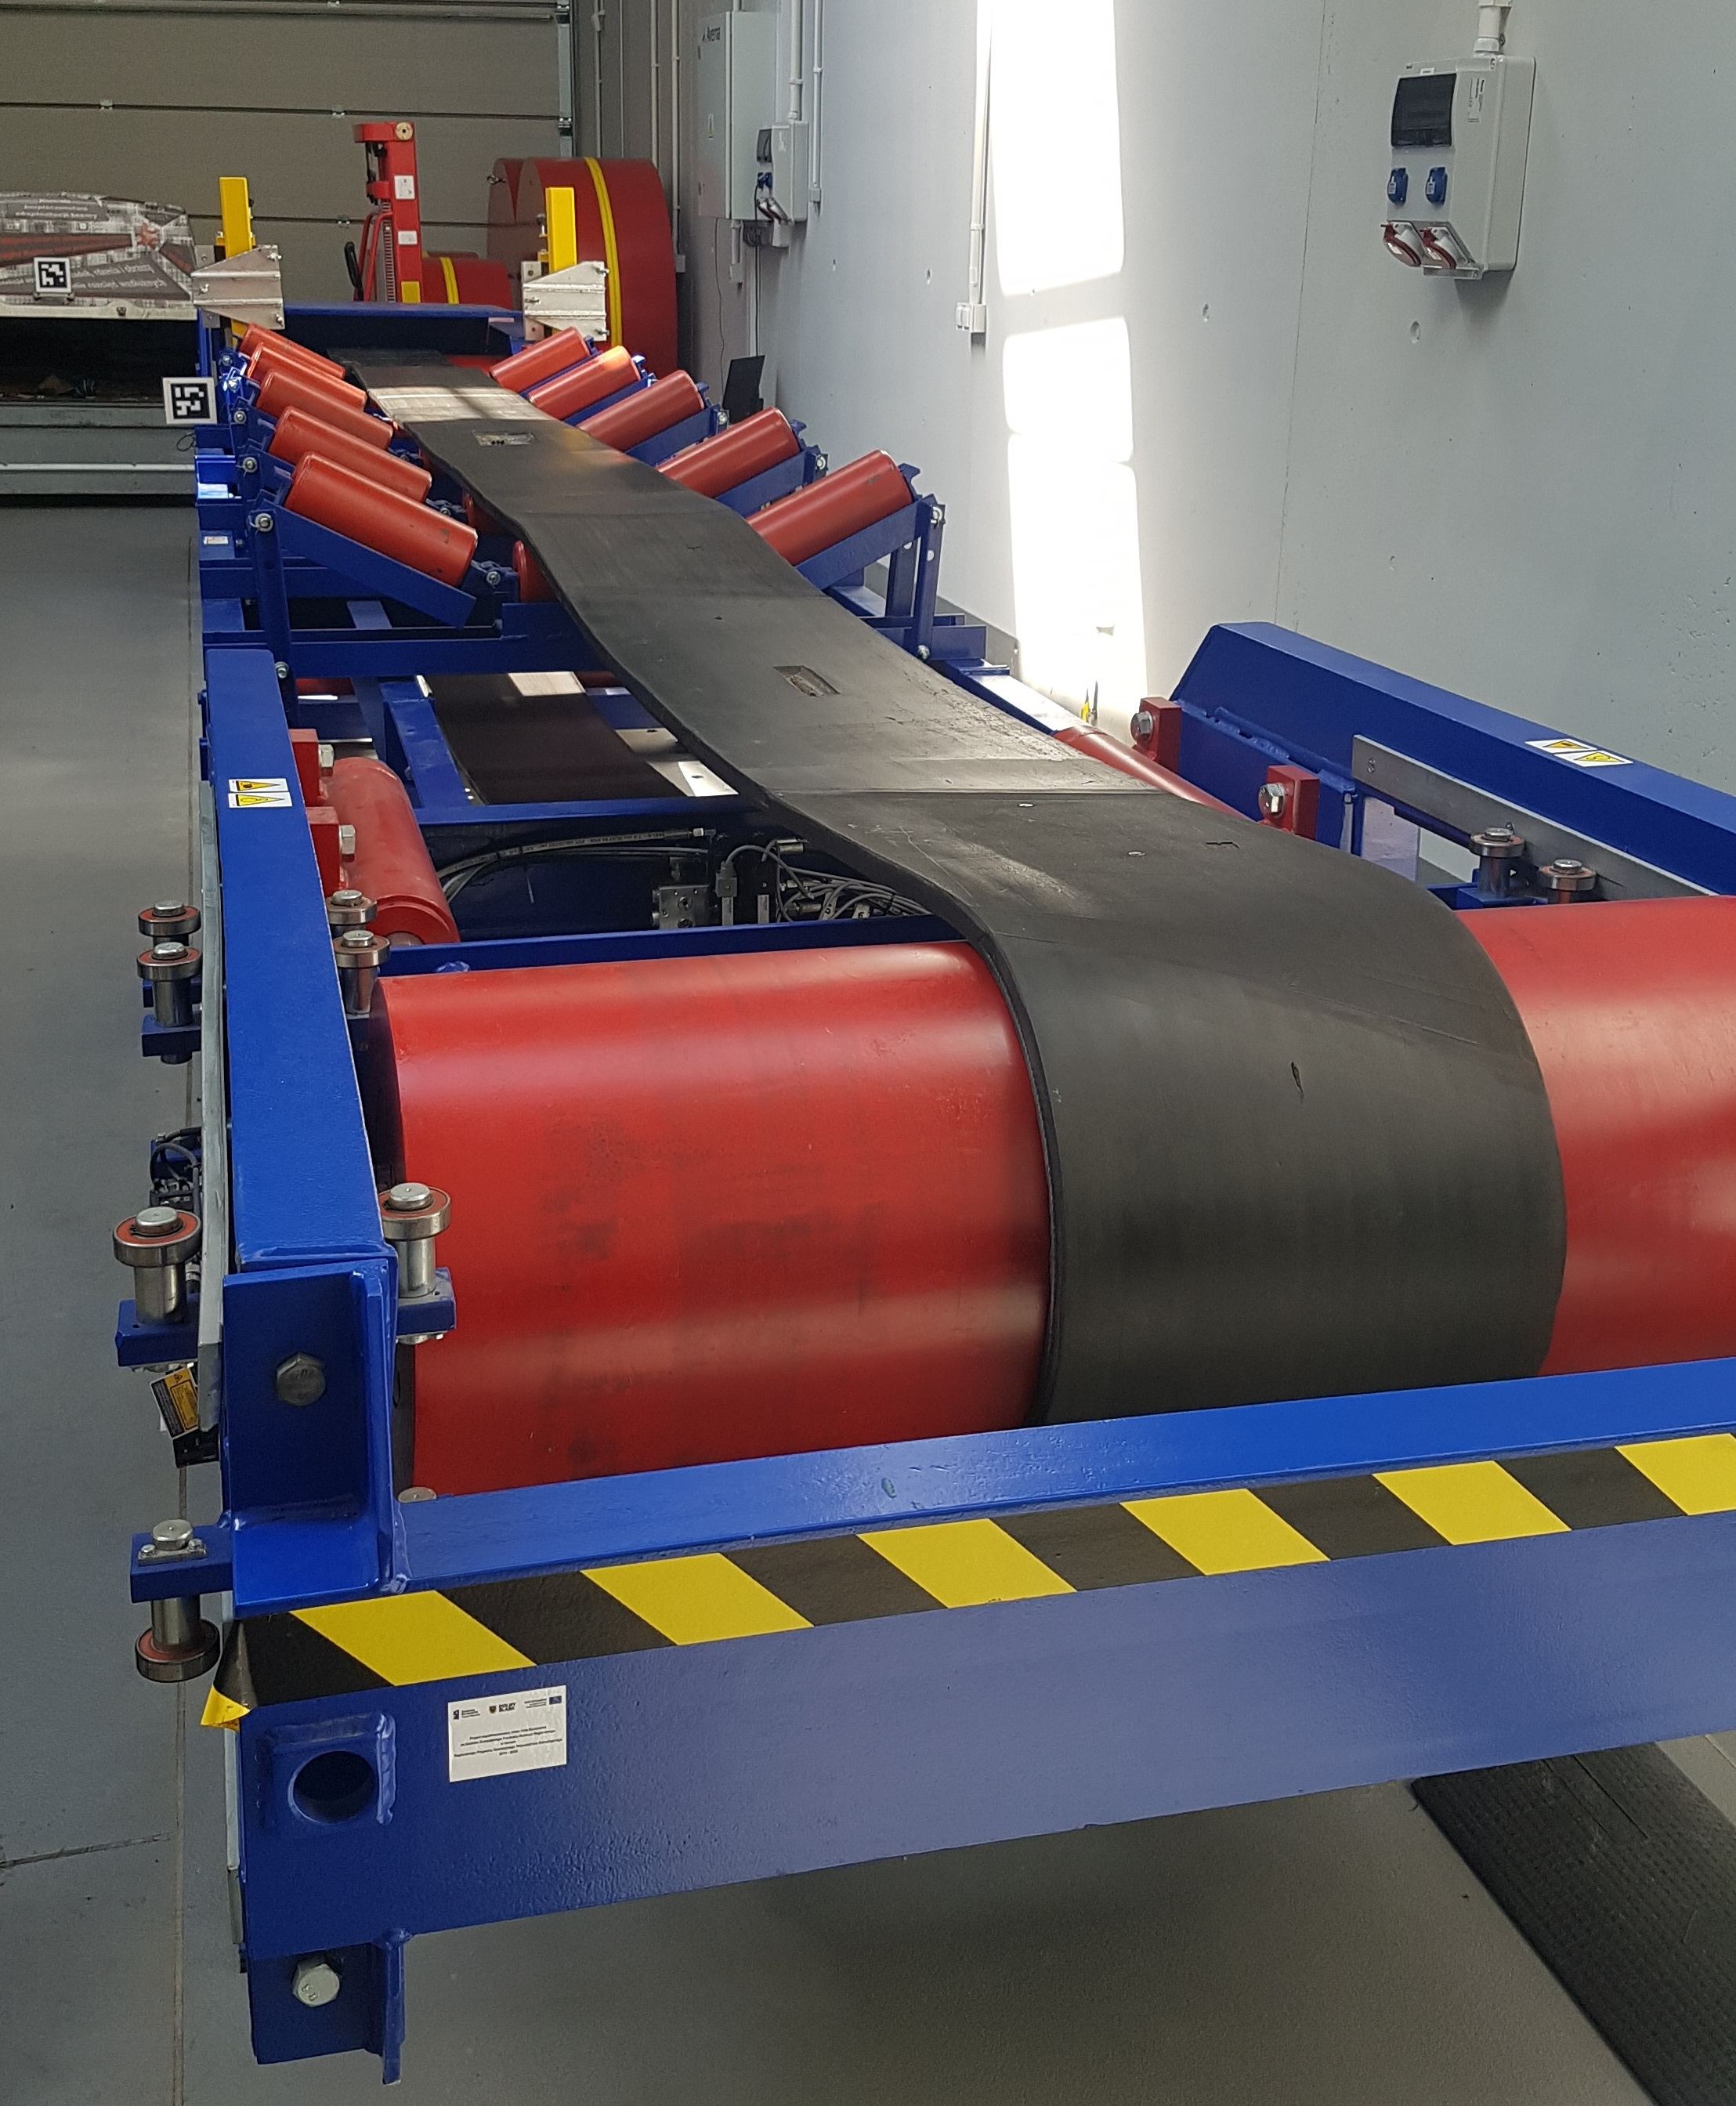
\includegraphics[width=0.4\textwidth, height=0.6\textwidth]{beltconveyor.jpg}
	\caption{Belt conveyor test rig in GEO3EM Research Center}
	\label{beltconveyor}
\end{figure}


\subsection{Plan of the experiment}
The experiment consisted of two components: traveling along a conveyor belt during his operation (see Fig. \ref{fig:plan_exp}, \ref{fig:robot_action}) and inspection data acquisition. 

\begin{figure}[ht!]
	\centering
	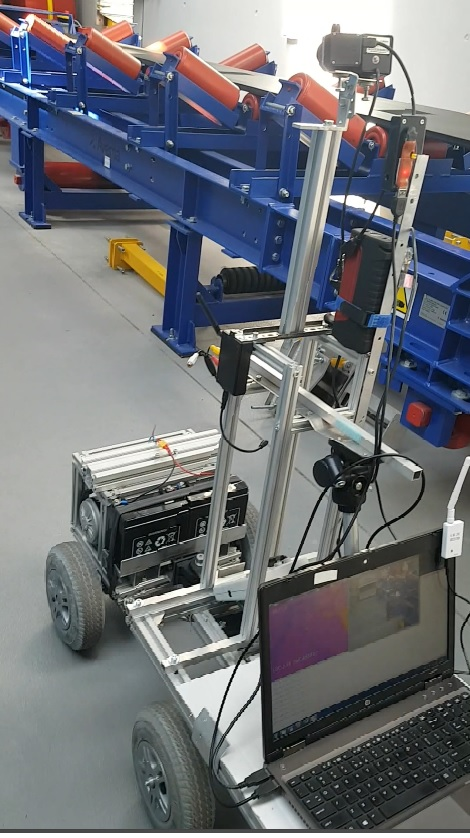
\includegraphics[width=0.3\textwidth]{measurement2.jpg}
	\caption{Robot in action - a view on a laptop screen}
	\label{fig:robot_action}
\end{figure}

\subsection{Results}
In this section we present results of experiments performed in lab conditions. In Fig \ref{fig:hot_idler} we present an infrared thermography image with one of idler with significantly higher temperature. At the same time RGB images have been acquired by the second camera. Hot areas detection was performed according to the algorithm presented in Fig. \ref{fig:alg_hot_detection}.



\begin{figure}[ht!]
	\centering
	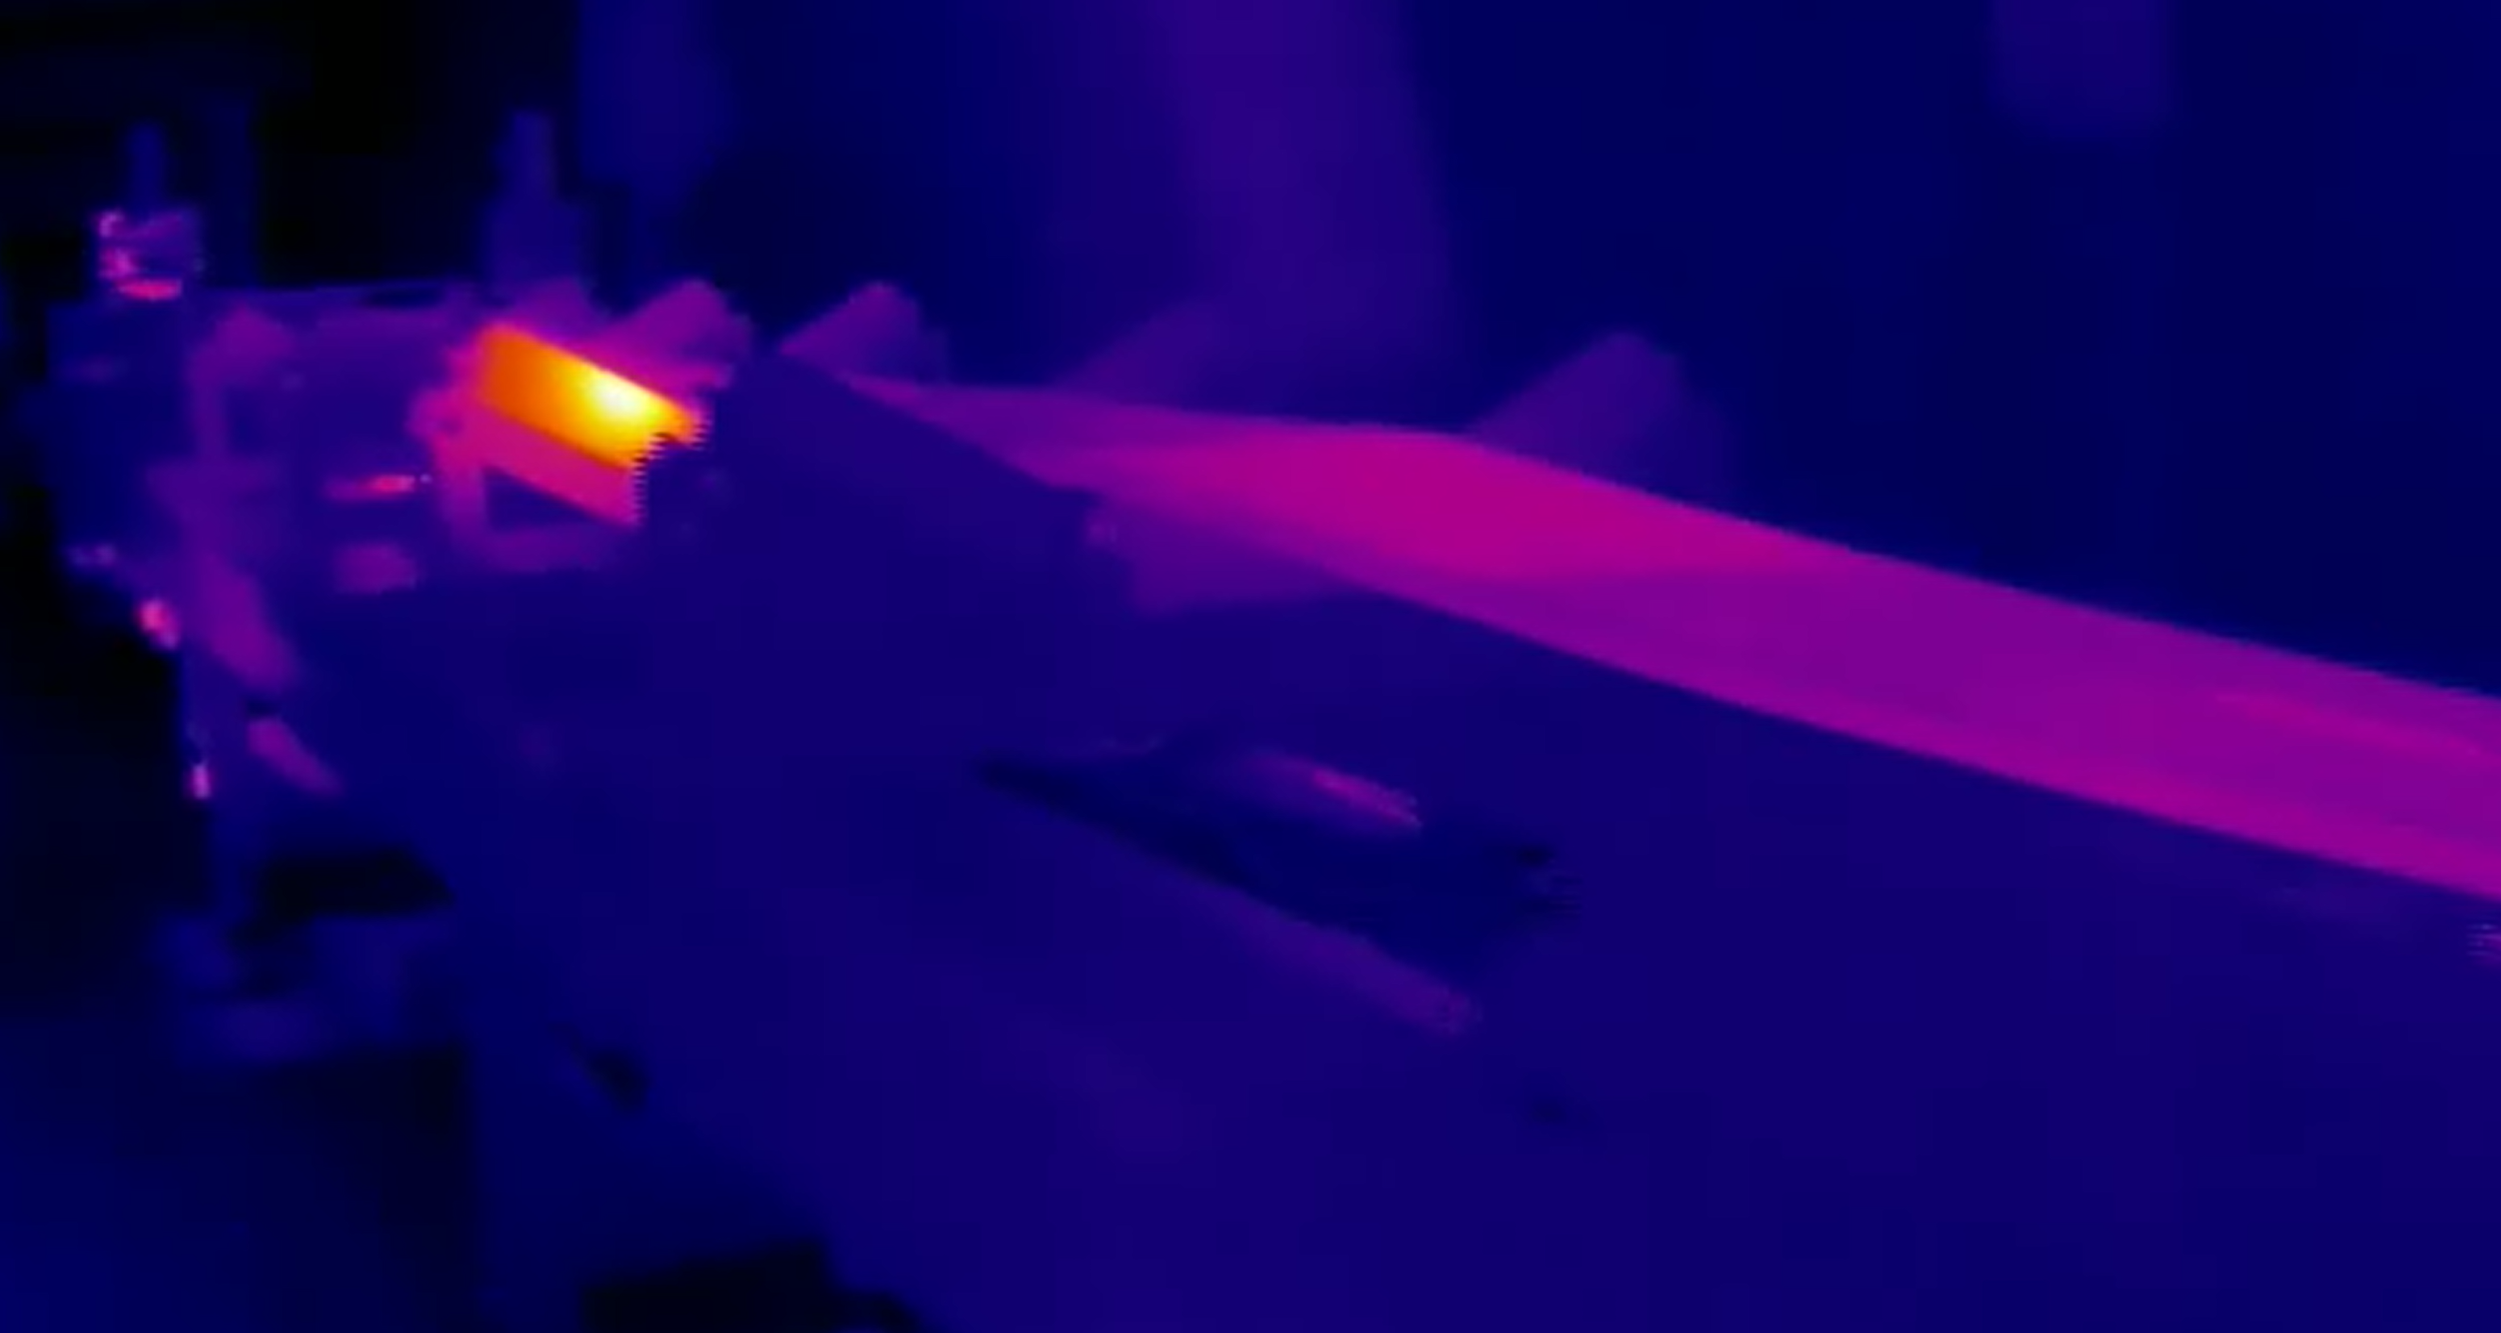
\includegraphics[width=0.7\textwidth]{hot_idler.png}
	\caption{An infrared thermography image with one of idler with significantly higher temperature.}
	\label{fig:hot_idler}
\end{figure}


\section{The inspection data processing - methods and results}
In this section we will present the results of our experiment in the lab as well as results of image processing and analysis. Our procedure consists of 3 steps: infrared image analysis, RGB image analysis, and fusion of these results to validate proper hot spot detection. 

\subsection{IR data processing for hot spot detection}

From image presented in Fig. \ref{fig:hot_idler} we have extracted a part of image with possible hot spot, see Fig. \ref{fig:termo}.
Using tools from Matlab (Image Segmentation Using the Color Thresholder App) we have segmented hot spot as presented in Fig.  \ref{fig:termo2}.

\begin{figure}
\centering
\begin{minipage}[c]{0.48\textwidth}
\centering
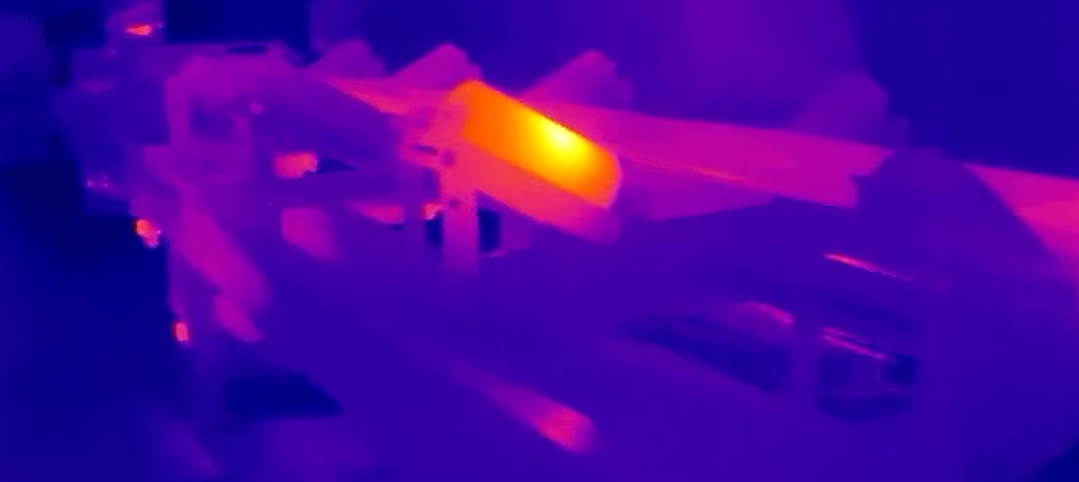
\includegraphics[width=6cm]{termo.png}
\centering
\caption{Localized neighbourhood of a hotspot.}
\label{fig:termo}
\end{minipage}
\hfill
\begin{minipage}[c]{0.48\textwidth}
\centering
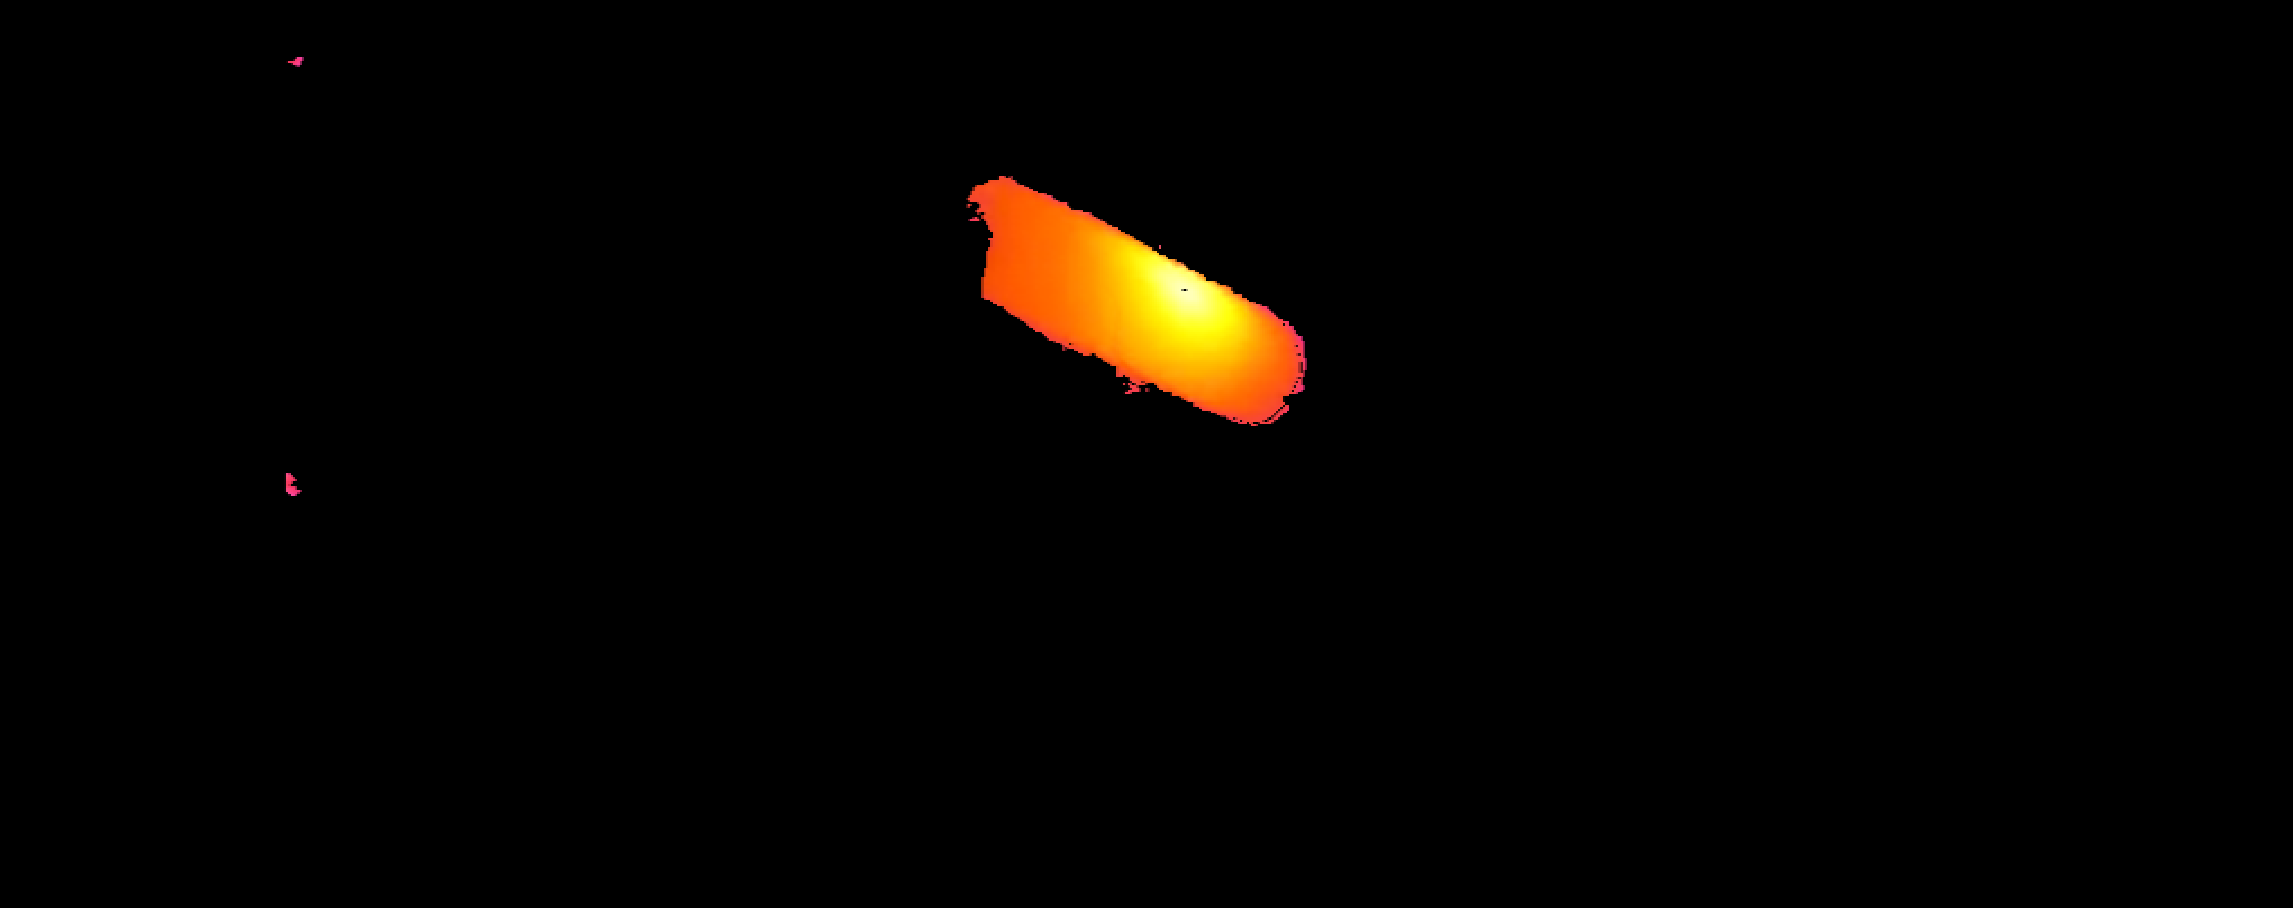
\includegraphics[width=6cm]{termo2.png}
\centering
\caption{Segmented hotspot.} \label{fig:termo2}
	
\end{minipage}
\end{figure}



\subsection{RGB image data processing for idler detection}

By analogy to the IR image, we have selected an RGB image with a belt conveyor on it. It was acquired at the same time as the IR image, with the same localization of robot. Using the same  Matlab tool as before (Image Segmentation Using the Color Thresholder App) we have segmented the image presented in Fig. \ref{fig:yyy} as presented in Fig. \ref{fig:yyy2}.

\begin{figure}
\centering
\begin{minipage}[c]{0.48\textwidth}
\centering

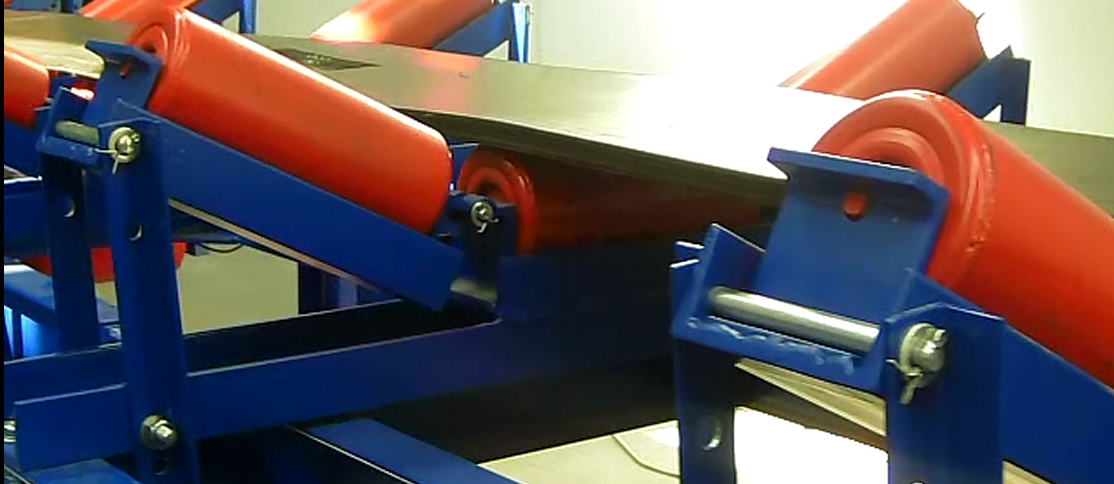
\includegraphics[width=0.6 \textwidth]{yyy.png}
	\caption{A Visual reference for hotspot localization.}
	\label{fig:yyy}


\end{minipage}
\hfill
\begin{minipage}[c]{0.48\textwidth}
\centering
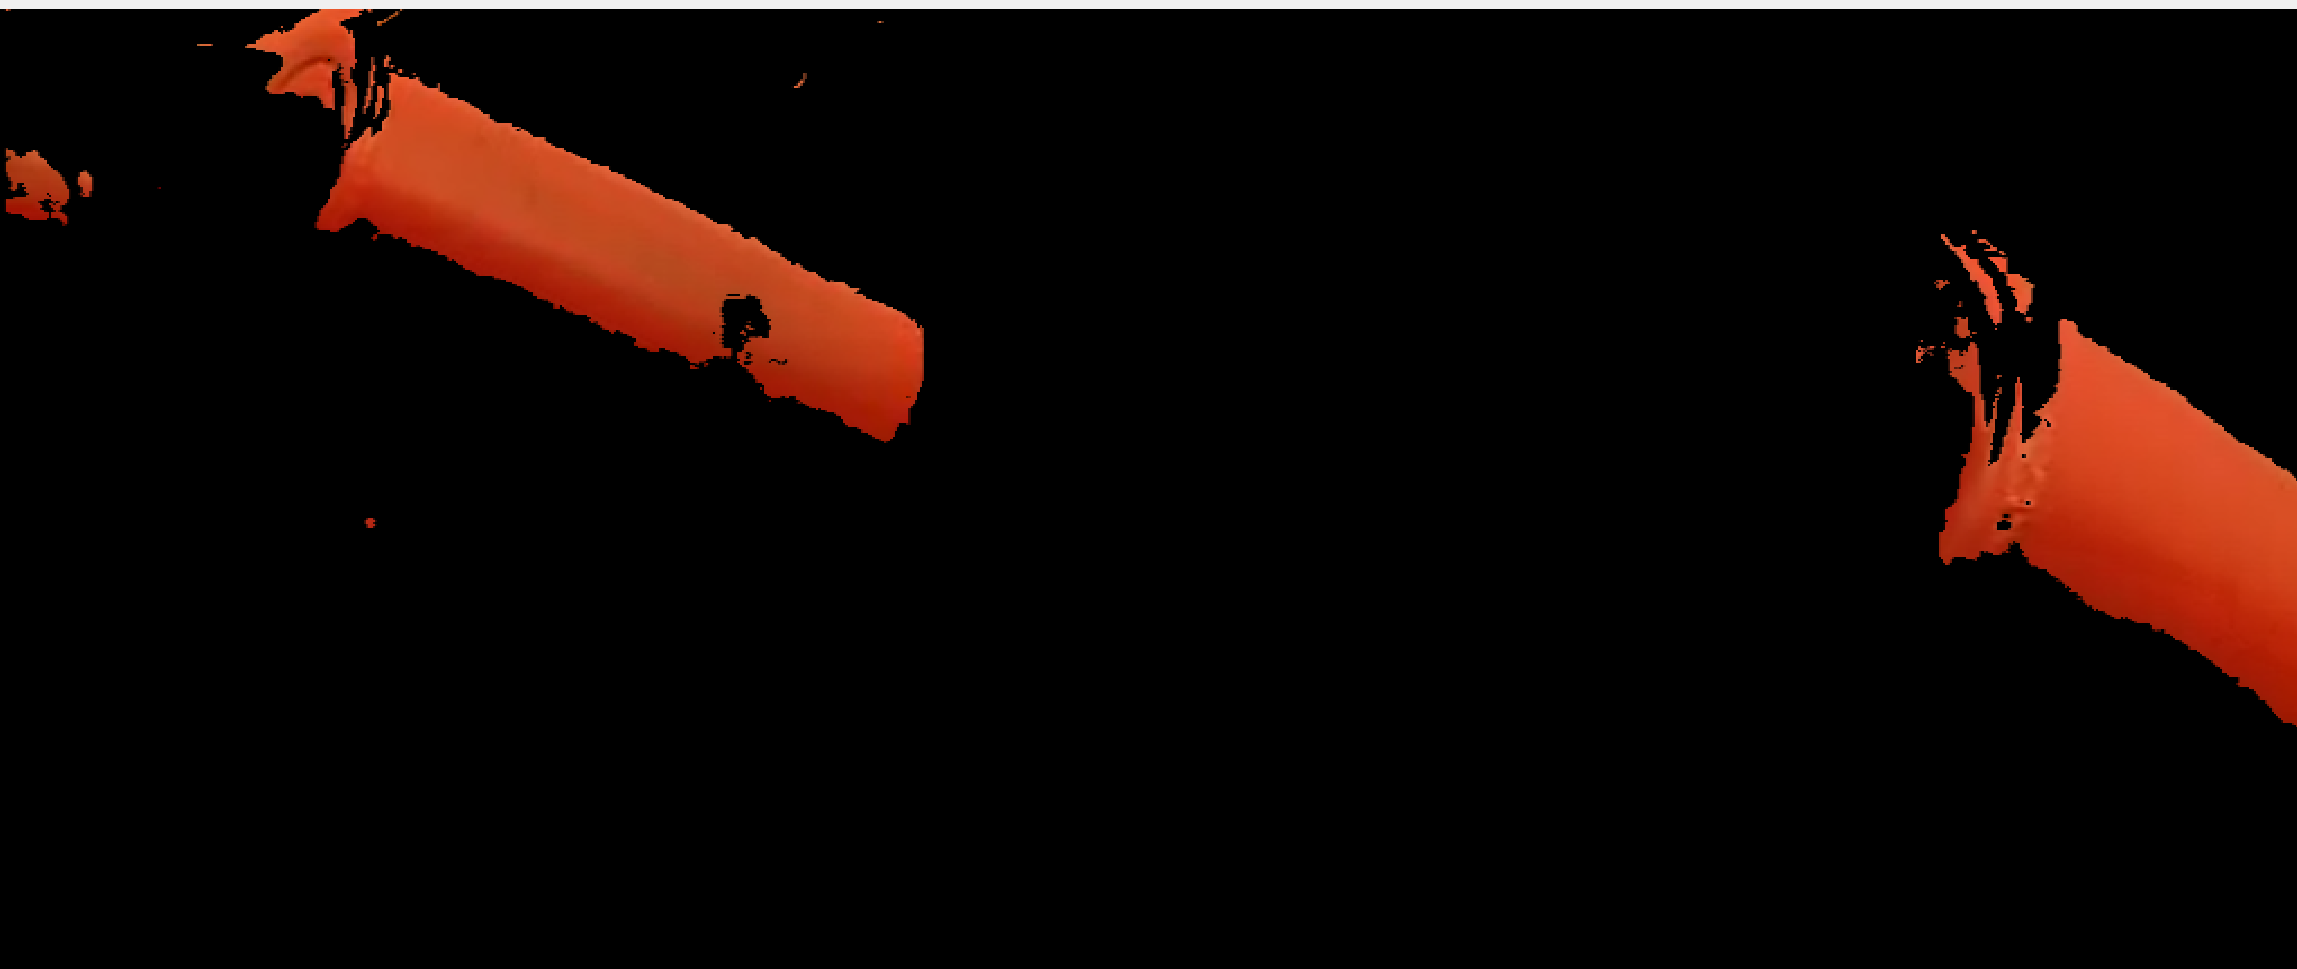
\includegraphics[width=0.8\textwidth]{yyy2.png}
	\caption{Segmented idlers.}
	\label{fig:yyy2}
	
\end{minipage}
\end{figure}




\subsection{The fusion of RGB image  and IR data processing for hot idler detection}
Along with the belt conveyor route one may detect many hot spots. To validate that detected hot spot as detected hot idler it is proposed to fuse RGB image and IR data. If segmented areas will be similar, one can conclude that detected hot spot is in fact the idler.
The idea of comparing two types of images is presented in Fig. \ref{fig:IRRGBfusion}.
In Fig. \ref{fig:fusion2} we present two segmented images. Based on shape and location we can confirm that the detected hot spot is a damaged idler.

\begin{figure}[ht!]
	\centering
	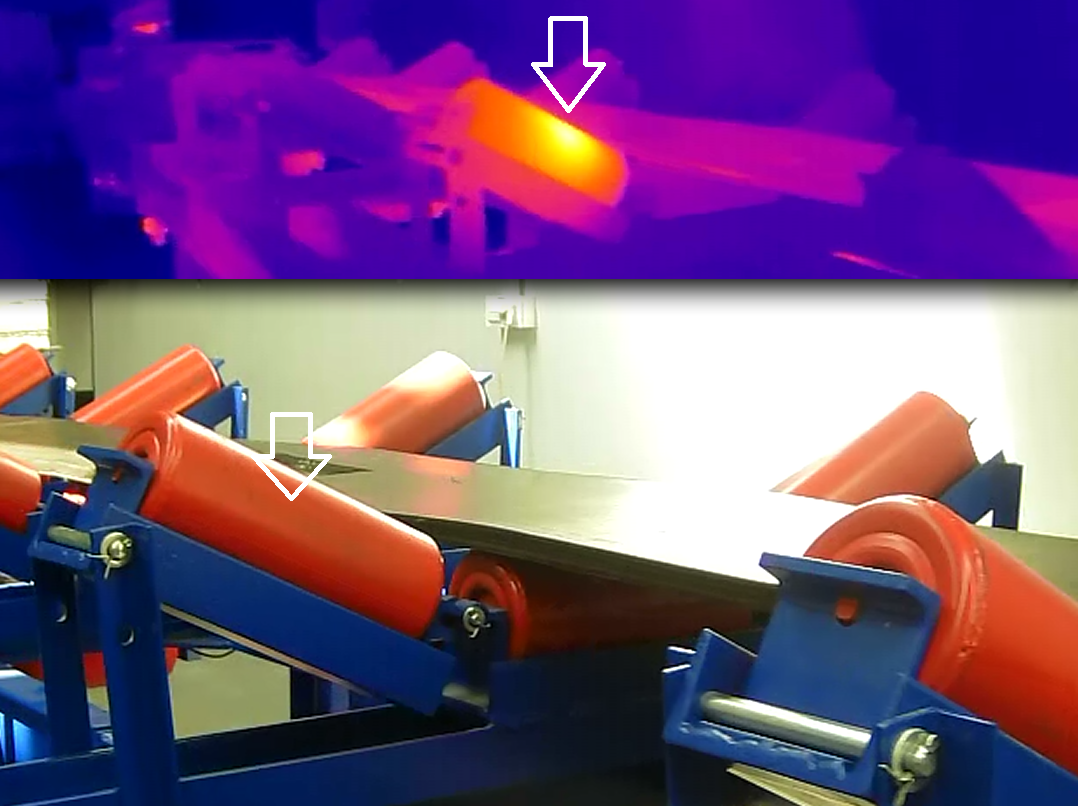
\includegraphics[width=0.5\textwidth]{IR_RGB fusion.png}
	\caption{An infrared thermography image and RGB image fusion for one of idler with significantly higher temperature.}
	\label{fig:IRRGBfusion}
\end{figure}

\begin{figure}[ht!]
	\centering
	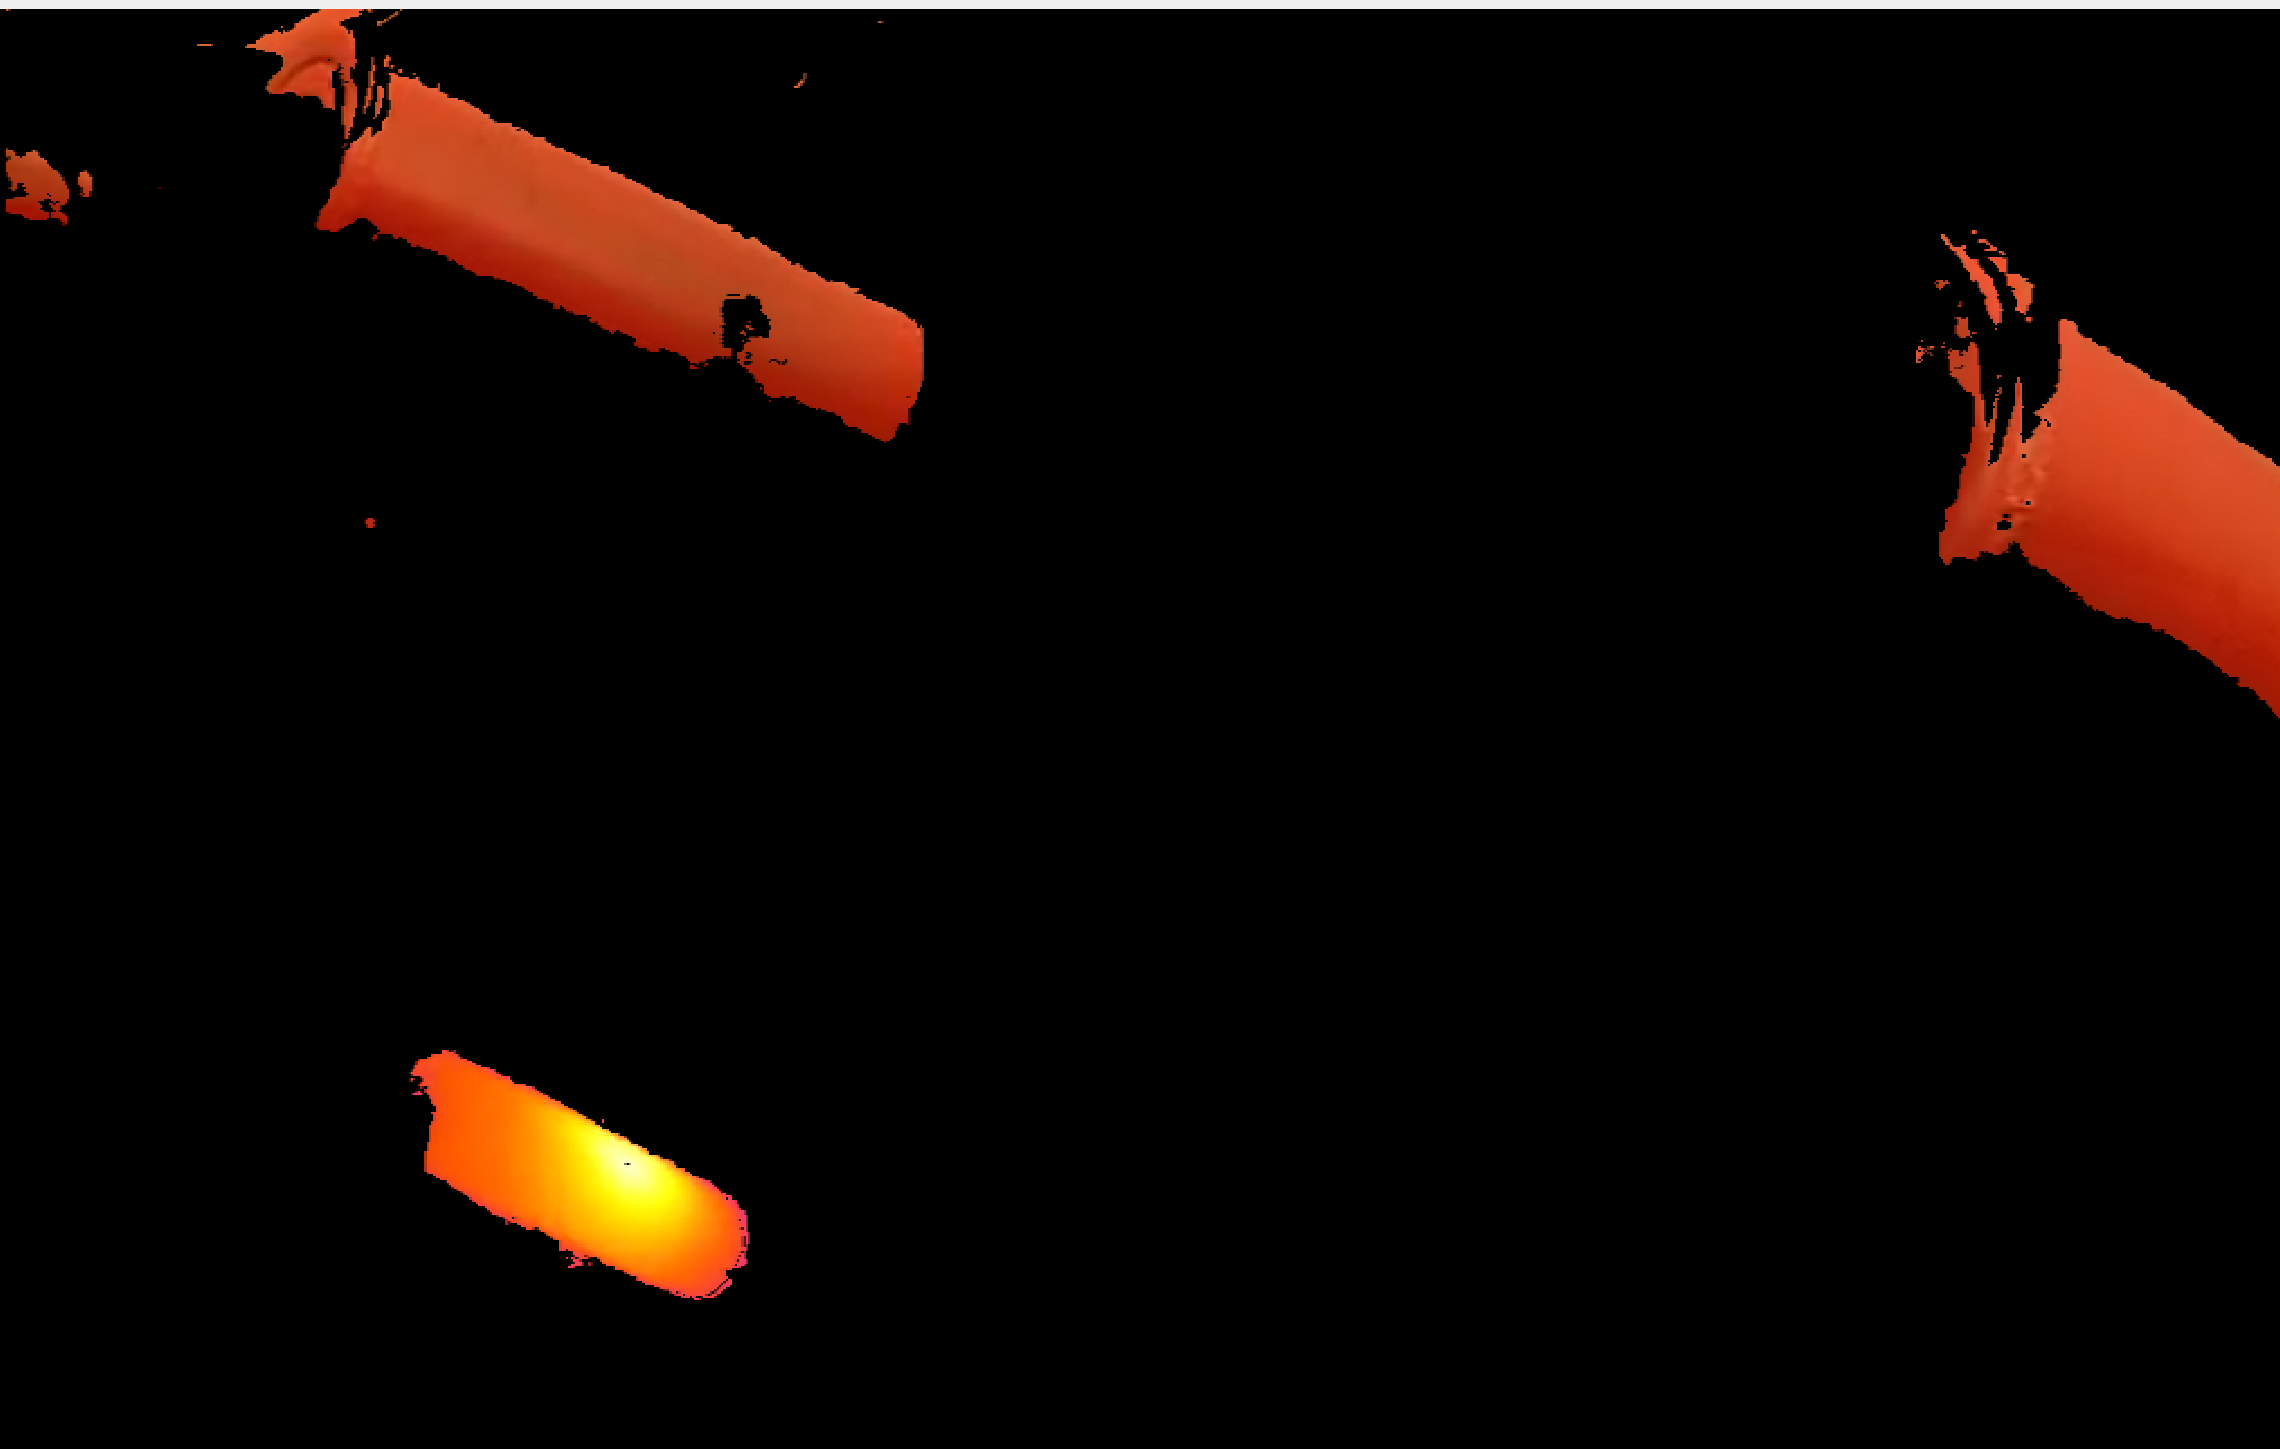
\includegraphics[width=0.5\textwidth]{fusion2.png}
	\caption{Result of infrared thermography image and RGB image fusion for one of idler with significantly higher temperature.}
	\label{fig:fusion2}
\end{figure}

\section{Discussion}\label{disc}
The experiment in the lab is usually an approximation of real environment use cases. Indeed, we are aware and we expect that the same experiment in the main will bring new challenges. However, we have checked, that usage infrared camera is possible and the quality of the IR picture is good enough to perform hot idler detection, see Fig. \ref{fig:BC_termo}.
In this figure, one may identify 3 idlers with higher temperatures (above the belt).
\begin{figure}[ht!]
	\centering
	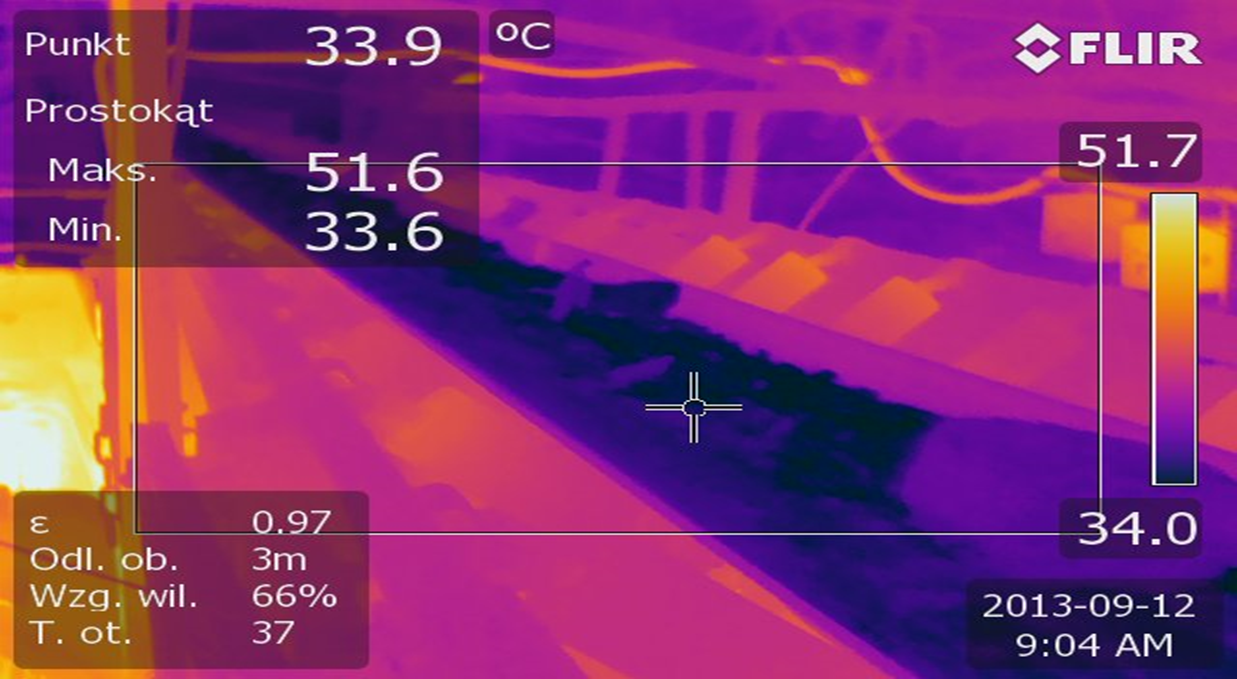
\includegraphics[width=0.8\textwidth]{BC_termo.png}
	\caption{Belt Conveyor as IR picture}
	\label{fig:BC_termo}
\end{figure}
The next step will be testing the prototype in the underground mine and collecting inspection data for various belt conveyors.

\section{Conclusions}
The UGV mobile robot has been proposed as a tool for inspection data collecting for belt conveyor maintenance. The robot, driven by a radio-based remote controller operated by humans was tested in lab conditions in the GEO3EM Research Center at Wroclaw University of Science and Technology. Artificially damaged idler (bearing fault) was introduced, so as a result we were able to use Infrared Thermography to identify hot spots along the conveyor route. The hot spot was detected using standard techniques for image segmentation available in Matlab software. The same approach has been used for idler detection using an RGB image. To validate that detected hot spot is the damaged idler, we fused an RGB image with an IR image. 
There is still a lot of work related to operator-human interaction or robot autonomy, locomotion of robot in the mining environment remains difficult. Automation of image analysis is also a challenge. However, we believe, that at this stage, we can send an inspection robot to do inspection in teleoperation mode along the conveyor route without human assistance. The mission could be limited to data acquisition, up to several hundred meters we can transmit data from robot to local computer at the beginning of the conveyor. Considering that the maximum length of the conveyor is 1000m - the inspection could be done in real-time if two access points (beginning and end of the conveyor route) are available. Knowing that each drive unit has sensors connected to SCADA - it is practically possible.

\section*{Author contributions}
Conceptualization, R.Z and J.S.; Methodology, R.Z and J.S. ; Investigation, J.S. J.W.and R.Z.
Mobile robot design, sensory system and software, J.S .; Idler detection software, R.Z.
Data acquisition software, J.S.; Writing original draft preparation, R.Z. and J.S.;
Formal analysis, R.B.; Writing review and editing, J.W.; Funding acquisition, R.Z. 
\section*{Founding}
This work is supported by EIT Raw Materials GmbH under the Framework Partnership Agreement
\section*{Acknowledgments}
This activity has received funding from the European Institute of Innovation and Technology (EIT), a body of the European Union, under the Horizon 2020, the EU Framework Programme for Research and Innovation. This work is supported by EIT Raw Materials GmbH under the Framework Partnership Agreement  (Autonomous Monitoring and Control System for Mining Plants - AMICOS).

\section*{Conflict of Interest}
The authors declare no conflict of interest.

%\section*{References}




% Hardware:
% \begin{itemize}
%     \item Układ zasilania (akumulatory i elektronika sterująca zasilaniem)
%     \item Układ jezdny/napędowy (koła, zawieszenie, silniki, mechanika skrętu kół, elektronika która tym steruje)
%     \item Układ komunikacji (anteny/ nadajniki i ich elektronika) do przesyłu danych lub sterowania z zewnątrz
%     \item Układ percpecji (czujniki nawigacyjne używane do poruszania się -- dalmierze, kamery, skanery itp)
%     \item Układ akwizycji danych (czujniki operacyjne)
% \end{itemize}

% Software:
% \begin{itemize}
%     \item Moduł sterowania lokomocji, obsługuje układ jezdny, komunikuje się z modułem nawigacji (autonomia) i modułem komunikacji (teleoperacja)
%     \item Moduł nawigacji (analiza i interpretacja otoczenia), obsługuje układ percepcji, komunikuje się z modułem sterowania
%     \item Moduł komunikacji, obsługuje układ komunikacji, komunikuje się z modułem sterowania i modułem przetwarzania danych
%     \item Moduł akwizycji i przetwarzania danych, obsługuje układ akwizycji danych, komunikuje się z modułem komunikacji
% \end{itemize}
% \end{thisnote}


\bibliography{mybibfile}

\end{document}